\documentclass[11pt,a4paper]{article}

\usepackage[margin=2.7cm,top=2.5cm,bottom=2.5cm]{geometry}
\usepackage[T1]{fontenc}
\usepackage[utf8]{inputenc}
\usepackage{newtxtext,newtxmath}
\usepackage{microtype}
\usepackage{amsmath}
\usepackage{booktabs}
\usepackage{graphicx}
\usepackage{siunitx}
\usepackage{xcolor}
\usepackage{natbib}
\usepackage{fancyhdr}
\usepackage{floatpag}
\usepackage{placeins}
\usepackage{titlesec}
\usepackage{enumitem}
\usepackage[
  font=small,
  labelfont=bf,
  justification=raggedright,
  singlelinecheck=false,
  skip=5pt
]{caption}
\usepackage{algorithm}
\usepackage{algpseudocode}
\usepackage{setspace}
\usepackage{hyperref}

\definecolor{OxfordBlue}{HTML}{002147}
\hypersetup{
  colorlinks=true,
  linkcolor=OxfordBlue,
  citecolor=OxfordBlue,
  urlcolor=OxfordBlue,
  pdftitle={Comparing protein sequence alignment score networks},
  pdfauthor={Davin (Haoping) Qiu}
}
\graphicspath{{figures/}}
% Generated by scripts/build_report_assets.py; do not edit by hand.
% Sources: dataset, experiment, score, graph-summary, null, and unweighted manifests/TSVs.
\newcommand{\MasterDomains}{960}
\newcommand{\MasterFamilies}{24}
\newcommand{\MasterClans}{8}
\newcommand{\MasterPairs}{460320}
\newcommand{\SampledCollections}{900}
\newcommand{\GraphsEvaluated}{21600}
\newcommand{\PrimaryCollections}{700}
\newcommand{\ExcludedCells}{4}
\newcommand{\ExcludedCollections}{200}
\newcommand{\PrimaryConditions}{14}
\newcommand{\ConditionCount}{18}
\newcommand{\ReplicatesPerCondition}{50}
\newcommand{\SamplingSeed}{20260828}
\newcommand{\TargetPerFamily}{40}
\newcommand{\BioTopFiveAMI}{0.938}
\newcommand{\BlastTopFiveAMI}{0.917}
\newcommand{\BioTopFiveClanAMI}{0.731}
\newcommand{\BlastTopFiveClanAMI}{0.705}
\newcommand{\BioTopTenAMI}{0.952}
\newcommand{\BlastTopTenAMI}{0.928}
\newcommand{\BioTopTenClanAMI}{0.772}
\newcommand{\BlastTopTenClanAMI}{0.734}
\newcommand{\BioPercentileNinetyClanAMI}{0.778}
\newcommand{\BlastPercentileNinetyClanAMI}{0.166}
\newcommand{\TopTenClanAMIGap}{0.006}
\newcommand{\TopFiveMinFamilyAMI}{0.917}
\newcommand{\BioTopFiveDensityPct}{4.18}
\newcommand{\BlastTopFiveDensityPct}{3.87}
\newcommand{\BioPercentileNinetyDensityPct}{10.00}
\newcommand{\BlastPercentileNinetyDensityPct}{0.83}
\newcommand{\MatchedTwoAbsDeltaNMI}{0.0034}
\newcommand{\MatchedTwoAbsDeltaAMI}{0.0094}
\newcommand{\SharedScoreSpearman}{0.976}
\newcommand{\ObservedTopFiveAMI}{0.936}
\newcommand{\NullTopFiveAMI}{0.009}
\newcommand{\UnweightedTopFiveAMI}{0.953}
\newcommand{\BlastPercentileNinetyNineNMI}{0.590}
\newcommand{\BlastPercentileNinetyNineAMI}{0.057}
\newcommand{\BlastPercentileNinetyNineCommunities}{150}
\newcommand{\BlastReportedPairs}{19376}
\newcommand{\BlastCoveragePct}{4.21}
\newcommand{\CompositionMinAMI}{0.883}
\newcommand{\CompositionMaxAMI}{1.000}
\newcommand{\BlastCompositionMinAMI}{0.879}
\newcommand{\BlastCompositionMaxAMI}{0.931}
\newcommand{\RepresentativeNodes}{160}
\newcommand{\RepresentativeFamilies}{8}
\newcommand{\RepresentativeBioEdges}{564}
\newcommand{\RepresentativeBlastEdges}{558}
\newcommand{\RepresentativeBioAMI}{0.958}
\newcommand{\RepresentativeBlastAMI}{0.958}
\newcommand{\RepresentativeBioComponents}{8}
\newcommand{\RepresentativeBlastComponents}{7}


\newcommand{\reportfooter}{%
  \fancyhf{}%
  \fancyfoot[C]{\small\thepage}%
  \renewcommand{\headrulewidth}{0pt}%
  \renewcommand{\footrulewidth}{0pt}%
}
\fancypagestyle{reportstyle}{\reportfooter}
\fancypagestyle{plain}{\reportfooter}
\pagestyle{reportstyle}
\floatpagestyle{reportstyle}
\setlength{\parindent}{1.5em}
\setlength{\parskip}{0pt}
\onehalfspacing
\titleformat{\section}{\color{OxfordBlue}\Large\bfseries}{\thesection}{0.5em}{}
\titleformat{\subsection}{\color{OxfordBlue}\large\bfseries}{\thesubsection}{0.45em}{}
\titlespacing*{\section}{0pt}{1.7em plus .2em minus .1em}{0.55em}
\titlespacing*{\subsection}{0pt}{1.2em plus .15em minus .1em}{0.35em}
\setlist[enumerate]{leftmargin=*,topsep=0.35em,itemsep=0.35em,parsep=0pt}
\setlength{\abovedisplayskip}{0.9em}
\setlength{\belowdisplayskip}{0.9em}
\setlength{\abovedisplayshortskip}{0.6em}
\setlength{\belowdisplayshortskip}{0.6em}
\setlength{\textfloatsep}{1.0em plus 0.15em minus 0.1em}
\setlength{\floatsep}{1.0em plus 0.15em minus 0.1em}
\setlength{\intextsep}{1.0em plus 0.15em minus 0.1em}
\renewcommand{\topfraction}{0.90}
\renewcommand{\bottomfraction}{0.80}
\renewcommand{\textfraction}{0.08}
\renewcommand{\floatpagefraction}{0.75}
\setcounter{topnumber}{3}
\setcounter{bottomnumber}{2}
\setcounter{totalnumber}{4}
\renewcommand{\arraystretch}{1.08}
\emergencystretch=2em
\widowpenalty=10000
\clubpenalty=10000
% forbid 1- and 2-line paragraph fragments, which float pressure in Results
% otherwise strands between figures
\widowpenalties 3 10000 10000 0
\clubpenalties 3 10000 10000 0
\raggedbottom
\sisetup{group-separator={,},group-minimum-digits=4}
\makeatletter
\setlength{\@fptop}{0pt}
\setlength{\@fpsep}{1.2em}
\setlength{\@fpbot}{0pt plus 1fil}
\setlength{\@dblfptop}{0pt}
\setlength{\@dblfpsep}{1.2em}
\setlength{\@dblfpbot}{0pt plus 1fil}
\makeatother

\begin{document}

\hypersetup{pageanchor=false}
\begin{titlepage}
  \thispagestyle{empty}
  \centering
  \vspace*{1.2cm}
  
\includegraphics[width=2.8cm]{logo2.png}\par
  \vspace{1.6cm}
  {\LARGE\bfseries Comparing protein sequence alignment score networks\par}
  \vspace{2.2cm}
  {\large Davin (Haoping) Qiu\par}
  \vspace{1.0cm}
  {\normalsize Supervisor: Karel Devriendt\par}
  \vspace{1.8cm}
  {\normalsize Mathematical Institute\par}
  \vspace{0.35em}
  {\normalsize University of Oxford\par}
  \vfill
  {\normalsize September 2026\par}
\end{titlepage}

\hypersetup{pageanchor=true}
\pagenumbering{arabic}
\setcounter{page}{1}

\section*{Abstract}
Sequence-similarity networks (SSNs) encode protein sequences as vertices and
selected pairwise similarities as edges. Their topology depends on the protein
sample, the score method, and the rule that turns scores into edges. We
systematically compare these methodological choices and evaluate how well the
resulting graph structure reflects Pfam protein families and clans. We
implemented a reproducible pipeline on \num{\MasterDomains} Pfam domains from
\MasterFamilies\ families and \MasterClans\ clans. Using a factorial design, we
sampled \num{\SampledCollections} balanced collections and built
\num{\GraphsEvaluated} weighted graphs from exact local alignment or BLAST
scores under three edge rule families, then detected communities with the
Louvain method. We measured recovery of withheld Pfam labels by adjusted mutual
information (AMI). Overall, top-\(k\) rules, which connect each domain to its
\(k\) highest-scoring neighbours, recovered Pfam structure most consistently
under both score methods; top-10 reached median family AMI \BioTopTenAMI\ with
exact alignment and \BlastTopTenAMI\ with BLAST. At matched 2\% edge density,
median absolute family normalised mutual information (NMI) difference between
methods was \MatchedTwoAbsDeltaNMI, whereas equal score percentiles produced
unequal densities.
Score permutation reduced family AMI at reference setting from
\ObservedTopFiveAMI\ to \NullTopFiveAMI. Results quantify sampling and edge
selection effects in protein network analysis.

\section{Introduction}

Proteins perform most molecular functions in living cells, including
catalysis, signalling, and transport. Proteins that share ancestry often share
structure and function, so relating proteins through their sequences is a basic
task in molecular biology.
We may consider a protein as a finite ordered sequence of amino-acid residues and
intuitively would expect proteins with similar sequences to be similar in some biological sense.
Protein alignment is then the family of techniques used to estimate ``similarity'' from amino acid
sequences alone \citep{durbin1998biological}. Protein sequences are typically long, so
we instead focus on protein domains: shorter, contiguous subsequences of a protein.

For any given pair of protein domain sequences of comparable length,
pairwise alignment inserts gaps into two such sequences so that residues judged
to correspond occupy shared positions; a gap marks residues present in one
sequence and absent in the other, an indel whose direction pairwise alignment
does not determine. A substitution matrix scores each aligned residue pair and
gap costs penalise indels, so total score rewards correspondence and penalises
 divergence. Global alignment scores two sequences over their full length;
local alignment selects one region of each sequence maximising total score, and
so tolerates unrelated flanking segments. Comparison at domain level uses local
alignment. Several algorithms produce such a score, differing in computational cost and in
which pairs they report; Section~\ref{sec:alignment_algo} discusses them further.

One application of pairwise alignment scores is the construction of
sequence-similarity networks (SSNs), in which vertices represent sequences and
selected pairs form weighted edges. SSNs support exploration and
clustering of protein families
\citep{atkinson2009sequence,gerlt2015efi,enright2002mcl}. Sequences alone do
not determine an SSN. Three choices intervene: the collection of proteins considered,
the alignment algorithm to score pairs, and the graph rule that promotes scores
to edges. Threshold choice has no accepted universal value, and reported
topology shifts with it \citep{apeltsin2011threshold,hornung2023objective}.

\medskip
In this article, we conduct a systematic comparison of methodological choices
in SSN construction. For graphs built from different protein collections,
alignment algorithms, and graph construction rules, we evaluate how well the
resulting graph structure reflects known biological protein families.

We vary these three choices systematically on a recorded panel of
\num{\MasterDomains} seed domains from \MasterFamilies\ families and
\MasterClans\ clans of the Pfam database \citep{mistry2021pfam}. Using a
factorial design, we sample \num{\SampledCollections} balanced collections, and
across two scoring methods and 12 edge settings we obtain
\num{\GraphsEvaluated} weighted graphs. We then detect communities in each graph
without using labels and quantify their agreement with withheld Pfam family and
clan labels.

\section{Alignment algorithms and scoring}
\label{sec:alignment_algo}

In this section, we describe the two methods we use to score pairs of
sequences: exact local alignment by the Smith--Waterman algorithm and heuristic
search by BLAST. We then compare their scoring systems and briefly describe a
learned alternative that we did not use at scale.

\subsection{Exact local alignment}
\label{ssec:exact}

Let \(x=x_1\ldots x_p\) and \(y=y_1\ldots y_q\) be amino-acid sequences,
where each \(x_i\) and \(y_j\) is one of the 20 standard amino acids.
A substitution matrix \(a(\cdot,\cdot)\) assigns score \(a(x_i,y_j)\) to an
aligned residue pair. BLOSUM62 is a \(20\times20\) substitution matrix
estimated from conserved blocks of aligned proteins, its entries scaled
log-odds of observed against chance residue pairing
\citep{henikoff1992amino}.

We use affine gap cost \citep{gotoh1982improved}, where opening a gap costs
\(g_o>0\) and each further gap residue costs \(g_e\), with \(0<g_e<g_o\), so a
gap of length \(\ell\) costs \(g_o+(\ell-1)g_e\). One long gap therefore costs
less than several short gaps of equal total length, since a single
multi-residue indel occurs more readily than several isolated ones. We take
\(g_o=11\) and \(g_e=1\), conventional values for BLOSUM62.

The Smith--Waterman algorithm finds an exact optimal local alignment by dynamic programming
\citep{smith1981identification}. Gotoh's formulation computes this optimum under
affine gap costs in \(O(pq)\) time by carrying separate states for gapped and ungapped
extensions,
\begin{align*}
E_{ij}&=\max\{H_{i-1,j}-g_o,\ E_{i-1,j}-g_e\},\\
F_{ij}&=\max\{H_{i,j-1}-g_o,\ F_{i,j-1}-g_e\},\\
H_{ij}&=\max\{0,\ H_{i-1,j-1}+a(x_i,y_j),\ E_{ij},\ F_{ij}\}.
\end{align*}
Here \(H_{ij}\) is best score of a local alignment ending with \(x_i\) aligned
to \(y_j\); \(E_{ij}\) is best score ending with \(x_i\) aligned to a gap in
\(y\); \(F_{ij}\) is best score ending with a gap in \(x\) aligned to \(y_j\).
Boundary values are \(H_{i0}=H_{0j}=0\), with gap states unavailable at a
boundary set to \(-\infty\). Zero inside \(H_{ij}\) lets an alignment restart,
which yields a local rather than global optimum. Under this recurrence a gap of
length \(\ell\) costs \(g_o+(\ell-1)g_e\), and local score is
\[
s(x,y)=\max_{i,j}H_{ij}.
\]
In this article, we compute exact local alignment scores with the
Smith--Waterman implementation in Biopython's \texttt{PairwiseAligner}
\citep{cock2009biopython}, run in local mode with BLOSUM62 and affine gap costs
\(g_o=11\) and \(g_e=1\).

\subsection{Heuristic search}
\label{ssec:heuristic}

BLASTP, the protein--protein search program of BLAST, avoids exhaustive dynamic programming. It indexes short words, locates
high-scoring word matches between query and subject, and extends only those
seeds into local alignments \citep{altschul1990basic,camacho2009blastplus}.
Cost per pair falls well below \(O(pq)\). A weakly similar pair may yield no
seed and therefore no reported alignment, so absence from BLAST output records
failure to reach a reporting threshold rather than a score of zero.

Raw score \(S\) carries units of its scoring system. Bit score rescales it to a scale independent of scoring system,
\[
S'=\frac{\lambda S-\log K}{\log 2},
\]
where \(\lambda\) and \(K\) are Karlin--Altschul parameters fixed by
substitution matrix, gap costs, and background residue frequencies
\citep{karlin1990methods}. In this article, BLAST graphs use bit scores \(S'\)
as edge weights.

We ran BLAST using BLOSUM62 and nominal gap costs \(g_o=11\) and \(g_e=1\), matching exact local
alignment of Section~\ref{ssec:exact}, so both methods score aligned residue
pairs from one substitution matrix. BLAST additionally applies
composition-based statistics in mode 2, which rescales substitution scores
separately for each query--subject pair according to that pair's residue
composition. Rescaling suppresses high scores arising from compositional bias
rather than from shared ancestry, for instance between two sequences that are both rich
in a single residue.

BLAST reports an alignment only when its expect value falls below a threshold.
For an alignment with raw score \(S\) and bit score \(S'\), the E-value of the pair is defined as
\[
E = K m'n'\,e^{-\lambda S} = m'n'\,2^{-S'},
\]
where \(m'\) and \(n'\) are effective query and database lengths after
correction for alignments truncated at sequence ends, and \(\lambda\), \(K\)
are as above. Both forms agree because \(2^{-S'}=Ke^{-\lambda S}\), the bit
score being defined precisely so that expect value takes this form. Hence \(E\)
counts alignments expected to reach score \(S\) by chance alone in a search of
that size, and small \(E\) marks a score unlikely to arise at random. Since
\(E\) scales with \(m'n'\), one value of \(E\) denotes different degrees of
similarity in databases of different size.

We used \(E=10\), the standard BLAST default. That value is permissive by
design, far above thresholds near \(10^{-3}\) conventionally used to claim
homology, and it exists to surface marginal hits rather than to establish
significance. Permissiveness is apt here since edge selection happens
downstream under rules of Section~\ref{sec:rules}, leaving \(E\) to determine
only which pairs carry a score at all.

BLAST searches are directional and may return several high-scoring segment
pairs (HSPs) for one query--subject comparison. HSP of highest bit score
represented each ordered pair, and highest score across reported directions
represented each unordered pair. In our experiments, BLAST reported \num{\BlastReportedPairs} of
\num{\MasterPairs} master pairs, or \(\BlastCoveragePct\%\).

\subsection{Comparability of the two scoring systems}

Both methods used BLOSUM62 and nominal gap parameters \(g_o=11\) and \(g_e=1\). Two
differences remain. BLAST charges an extension cost for every gap residue, so a
gap of length \(\ell\) costs \(g_o+\ell g_e\), exceeding cost under exact alignment by
\(g_e\) at every gap. Composition-based statistics further adjust BLAST
substitution scores per sequence pair, while exact local alignment applies one
fixed matrix throughout.

Each method therefore ran at its own standard default. Method comparisons in
this report control vertex set and edge count (Section~\ref{sec:rules}) rather
than assert identical scoring systems.

\subsection{Learned alignment}

DEDAL is a pretrained neural model that learns sequence representations and
alignment parameters from protein data, returning a Smith--Waterman-style score
\citep{llinareslopez2023deep}. We verified this pretrained model on pilot data,
but its measured runtime exceeded our compute budget for all-versus-all scoring
of the master panel (Section~\ref{ssec:panel}), so scaled results use exact
local alignment and BLAST only.

\section{Methods}

In this section, we describe how we turn pair scores into graphs and evaluate
them. We first define networks built from pair scores, then describe how we
select a panel of Pfam domains and sample collections from it, how edge rules
select edges, and how we detect communities and compare them with Pfam labels.

\subsection{Networks from pair scores}

A collection \(C\) is a set of protein domain sequences drawn from the master
panel (Section~\ref{ssec:panel}). Each graph built from \(C\) has one vertex
per sequence, so we identify its vertex set \(V\) with \(C\). Let \(n=\lvert V\rvert\),
\(\mathcal P(V)=\{\{i,j\}:i,j\in V,\ i\neq j\}\), and
\(P=\lvert\mathcal P(V)\rvert=\binom n2\). Method \(m\) reports score
\(s_e^m\) for each pair in available set \(A_m\subseteq\mathcal P(V)\); pairs
outside \(A_m\) stay missing and never receive an imputed value. Edge setting
\(\theta\) selects \(E_{m,\theta}\subseteq A_m\), giving weighted graph
\[
G(C,m,\theta)=(V,E_{m,\theta},w_m),\qquad w_m(e)=s_e^m,
\]
with realised density \(\delta=\lvert E_{m,\theta}\rvert/P\), fraction of
possible pairs that became edges. Term \emph{realised} marks \(\delta\) as an
outcome rather than an input, since top-\(k\) and percentile rules fix no edge
count in advance and target density can fall short of its request. Every input
sequence remains a vertex; sequences with no selected pair become isolated vertices.

Each vertex carries a stable identifier formed from its UniProt accession with
domain start and end coordinates, for example \texttt{A0A0H3GJZ1\_27\_153}.
Lexicographic order of identifiers resolves ties wherever a selection would
otherwise be ambiguous, making every procedure below deterministic.

The path from collection to reported quantity is
\[
C \longrightarrow \{s_e^m:e\in A_m\}
\longrightarrow G(C,m,\theta)
\longrightarrow U(C,m,\theta)
\longrightarrow \operatorname{AMI}(U,V^*),
\]
where \(U\) is a community partition detected without labels and \(V^*\) is
withheld Pfam partition. The remaining subsections define each arrow. The master panel
and sampling design fix \(C\), edge rules fix \(\theta\), and community
detection with agreement measures fixes \(U\) and final comparison.

\subsection{Master panel}
\label{ssec:panel}

To sample subsets of protein sequences on which to build graphs, we first fix a
master panel: a recorded set of Pfam seed domains from which every collection is
drawn. The Pfam database defines families of homologous domains using curated seed alignments and
profile hidden Markov models; clans group families with evidence of common
ancestry \citep{mistry2021pfam}.

We select the panel by a rejection sampling procedure over Pfam clans. The
procedure first reads the official family--clan catalogue, discards
unassigned families and clans holding fewer than three catalogue families, then
shuffles the sorted clan list. Within each clan in that order it shuffles the sorted
family list and inspects families in turn, accepting those of InterPro type
\emph{domain} or \emph{family} carrying at least \TargetPerFamily\ reported
seed domains. A clan is retained once three families are accepted, and skipped
when fewer prove eligible. Selection stops at \MasterClans\ retained clans. One
random stream drives every shuffle, so a single seed reproduces the panel. A trace
table records every family inspected together with its acceptance or rejection. Pseudocode of the full procedure
may be found in Appendix~\ref{app:panel}.

Each selected seed alignment is filtered to unique sequences over 20 standard
amino acids with consistent coordinates. We then use deterministic farthest-point sampling
to select \TargetPerFamily\ representatives per family. First sequence has
length nearest family median. Given selected set \(S\) and remaining set
\(R\), next sequence is
\[
x^*=\arg\max_{x\in R}\min_{y\in S}d(x,y),\qquad
d(x,y)=1-\operatorname{identity}(x,y),
\]
where identity counts matching residues over jointly occupied seed alignment
positions. Identifier order resolves ties. This maximises within-family
sequence diversity, so recovery results are conservative relative to a
sample of each family weighted by frequency. Alignment gaps are removed before
scoring. Panel contains \num{\MasterDomains} domains, \MasterFamilies\
families, \MasterClans\ clans, and
\(\binom{\MasterDomains}{2}=\num{\MasterPairs}\) unordered pairs.

\subsection{Repeated collections}

Each collection is a balanced hierarchical draw. For condition \((c,f,r)\),
sample \(c\) clans uniformly without replacement, then \(f\) families within
each selected clan, then \(r\) domains within each selected family. Collection
size is \(n=cfr\), with equal family sizes by construction. Factor levels are
\[
c\in\{2,4,8\},\qquad f\in\{2,3\},\qquad r\in\{10,20,40\}.
\]
Cartesian product gives \(3\cdot2\cdot3=\ConditionCount\) conditions, and
\ReplicatesPerCondition\ seeded replicates per condition give
\(\ConditionCount\cdot\ReplicatesPerCondition=\SampledCollections\) collection
declarations. A stable hash of base seed, condition, and replicate index
generates each replicate seed, so extending the design leaves earlier
collections unchanged. Pfam labels determine sampling strata and are then
withheld; they enter no score, edge rule, or community detection.

Conditions requesting most of the panel can repeat a complete node set across
replicates despite distinct seeds. A uniqueness audit hashes sorted node
identifiers within each condition. \ExcludedCells\ conditions contain
duplicates; their \ExcludedCollections\ declarations remain in audit tables and
figures but leave distributional summaries. Primary distributions therefore use
\PrimaryCollections\ collections from \PrimaryConditions\ conditions with
\ReplicatesPerCondition\ distinct node sets each. All \ExcludedCells\ excluded
conditions request \(r=40\), so exclusion falls entirely on largest domain
count and composition effects reported below are conservative. Two score
methods and 12 edge settings generate \num{\GraphsEvaluated} graphs before this
filter.

\subsection{Edge rules}
\label{sec:rules}

Recall vertex set \(V\) of collection \(C\), possible pairs \(\mathcal P(V)\)
with \(P=\lvert\mathcal P(V)\rvert\), and available set
\(A_m\subseteq\mathcal P(V)\) of pairs that method \(m\) scores. Edge setting
\(\theta\) is a rule family together with its parameter, taking one of forms
\((\mathrm{top},k)\), \((\mathrm{pct},p)\), or \((\mathrm{dens},d)\) defined
below.

For \(i\in V\), the available neighbours are \(A_m(i)=\{j\in V:\{i,j\}\in A_m\}\). Let \(N_k^m(i)\) be the
first \(\min\{k,\lvert A_m(i)\rvert\}\) elements of
\(A_m(i)\) under descending score with ties broken by ascending identifier. For
\(e\in A_m\), let \(r_e^m\in(0,1]\) be the ascending rank of \(s_e^m\), with ties
averaged and divided by \(\lvert A_m\rvert\), and let \(q_e^m\) be the descending rank,
with \(q_e^m=1\) at highest score. Let
\(b_m(d)=\min\{\lvert A_m\rvert,\lceil dP\rceil\}\). Three rule families are
\begin{align*}
E_{m,k}^{\mathrm{top}}
  &=\{e=\{i,j\}\in A_m:j\in N_k^m(i)\text{ or }i\in N_k^m(j)\},\\
E_{m,p}^{\mathrm{pct}}
  &=\{e\in A_m:r_e^m\geq p\},\\
E_{m,d}^{\mathrm{dens}}
  &=\{e\in A_m:q_e^m\leq b_m(d)\}.
\end{align*}
\(E_{m,k}^{\mathrm{top}}\) (top, \(k\)) lets each vertex nominate up to \(k\) strongest available neighbours
and retains undirected union, so retained edge count grows with \(n\) rather
than with \(\binom n2\) \citep{camoglu2006multiattribute}. \(E_{m,p}^{\mathrm{pct}}\) (pct, \(p\))
retains the upper tail of scores a method reported, so it acts on \(A_m\); it
coincides with target density \(1-p\) exactly when \(A_m=\mathcal P(V)\), and
otherwise yields a sparser graph in proportion to missing coverage. \(E_{m,d}^{\mathrm{dens}}\) (dens, \(d\)) requests a common global edge budget \(\lceil dP\rceil\) on
identical vertex sets, with shortfall
\(\max\{0,\lceil dP\rceil-\lvert A_m\rvert\}\) recording a budget a method
could not supply. The parameters used in our experiments are
\[
k\in\{1,2,5,10\},\qquad
p\in\{0.90,0.95,0.98,0.99\},\qquad
d\in\{0.005,0.01,0.02,0.05\},
\]
giving 12 settings per method.

\subsection{Communities and agreement}

To find groups of vertices that are densely connected to each other, we apply
community detection to each graph. Several methods exist; we use the Louvain
method. We identified communities in the graphs using weighted Louvain
optimisation \citep{blondel2008fast}, as implemented in NetworkX
\citep{hagberg2008exploring}. This heuristic starts with each vertex in its own
community and alternates two phases. First, it moves single vertices into a
neighbouring community whenever the move increases weighted modularity; second,
it merges each community into a single vertex and repeats on the reduced graph,
stopping when no move increases modularity. Weighted modularity is
\[
Q=\frac{1}{2W}\sum_{i,j}\left(w_{ij}-\gamma\frac{k_i k_j}{2W}\right)
\mathbf 1\{u_i=u_j\}.
\]
For vertices \(i\) and \(j\), \(w_{ij}\) is their edge weight when
\(\{i,j\}\in E\), and zero otherwise. Weighted degree is
\(k_i=\sum_j w_{ij}\), and total edge weight is
\(W=\frac12\sum_{i,j}w_{ij}\). The parameter \(\gamma>0\) controls community
resolution; all experiments use \(\gamma=1\). Variable \(u_i\) denotes the
community assigned to vertex \(i\), hence indicator \(\mathbf1\{u_i=u_j\}\) equals
one when \(i\) and \(j\) share a community.

To compare detected community structure with ground-truth Pfam family and
clan labels, we use two measures: normalised mutual information (NMI) and
adjusted mutual information (AMI). Choose one of \(n\) vertices uniformly. Let \(U\) be its detected community and
\(V^*\) its withheld Pfam label. Let \(n_{uv}\) count vertices assigned to
community \(u\) with label \(v\), \(n_u=\sum_v n_{uv}\), and
\(n_v=\sum_u n_{uv}\). Joint and marginal proportions are
\[
p_{uv}=\frac{n_{uv}}n,\qquad
p_u=\frac{n_u}n=\sum_v p_{uv},\qquad
p_v=\frac{n_v}n=\sum_u p_{uv}.
\]
Define
\[
I(U;V^*)=\sum_{u,v}p_{uv}\log\frac{p_{uv}}{p_u p_v},\qquad
H(U)=-\sum_u p_u\log p_u,\qquad
H(V^*)=-\sum_v p_v\log p_v,
\]
with \(0\log0=0\); \(\log\) denotes natural logarithm. NMI and AMI are defined as
\begin{align*}
\operatorname{NMI}(U,V^*)&=\frac{I(U;V^*)}{[H(U)+H(V^*)]/2},\\
\operatorname{AMI}(U,V^*)&=
\frac{I(U;V^*)-\mathbb E[I(U;V^*)]}
{[H(U)+H(V^*)]/2-\mathbb E[I(U;V^*)]}.
\end{align*}
Expectation averages mutual information over random contingency tables with
observed row and column margins fixed. NMI lies in \([0,1]\) and rises with
partition count even under independence, since a finer partition raises
\(I(U;V^*)\) by chance alone. AMI subtracts that expectation, takes value
\(0\) in expectation under independence, and so permits comparison across
settings whose community counts differ \citep{vinh2010information}. We computed
both NMI and AMI using scikit-learn \citep{pedregosa2011scikitlearn}. We stress
again that family and clan labels entered evaluation only after community
detection.

\subsection{Reproducibility and figure provenance}

Stored graph tables carry one row per graph and reference label level, and all
reported analyses read those tables. Script
\path{scripts/build_report_assets.py} generates every figure and numerical
macro from saved TSV and JSON artifacts. Canonical PNGs are written under
\path{outputs/figures/pfam_large_panel_report/}; identical copies are
placed in \path{report/figures/}. File \path{report/figure_provenance.tsv} maps
each image to its generating script, exact input tables, both paths, and
SHA-256 checksum. Report prose imports generated macros from
\path{report/generated_results.tex}, so no numerical result is transcribed by
hand.

\section{Results}

Our analysis centres on which edge rule yields communities closest to withheld
Pfam structure. Agreement with Pfam labels serves as a proxy, however limited,
for how well graph structure reflects biological information. We compared each
Louvain partition separately with family and clan assignments. We evaluate each
tested setting by median AMI across \PrimaryCollections\ distinct primary
collections; NMI shows the effect of chance correction. We report medians
rather than means because both measures are bounded and their replicate
distributions are asymmetric: several settings concentrate against 0 or 1, and
some are multimodal (Figs.~\ref{fig:nmi-frequency} and~\ref{fig:ami-frequency}).
The median is less sensitive to this skew and to outlying replicates.
Figures report interquartile ranges across collections as error bars. Detailed distribution plots use reference condition
\((c,f,r)=(4,2,20)\): \ReplicatesPerCondition\ collections, each containing 160
domains from 8 families.

\subsection{Graph-rule recovery of Pfam structure}

Figure~\ref{fig:rules} gives median AMI against median realised density. Family
recovery increased from top-1 to top-10 under both score methods. Top-10 gave
highest tested family AMI: \BioTopTenAMI\ for Biopython and \BlastTopTenAMI\ for
BLAST. Corresponding clan AMI was \BioTopTenClanAMI\ and
\BlastTopTenClanAMI. Biopython percentile 0.90 gave clan AMI
\BioPercentileNinetyClanAMI, exceeding Biopython top-10 by
\TopTenClanAMIGap; its BLAST counterpart gave
\BlastPercentileNinetyClanAMI. Top-10 was therefore first or within
\TopTenClanAMIGap\ of first for both label levels and both score methods.

Top-5 supplied a lower-density operating point. Median family AMI was
\BioTopFiveAMI\ for Biopython and \BlastTopFiveAMI\ for BLAST at densities
\BioTopFiveDensityPct\% and \BlastTopFiveDensityPct\%. Median clan AMI was
\BioTopFiveClanAMI\ and \BlastTopFiveClanAMI. Subsequent examples use top-5 to
retain fewer edges; the smaller of the two median family AMI values is
\TopFiveMinFamilyAMI.

\begin{figure}[htbp]
  \centering
  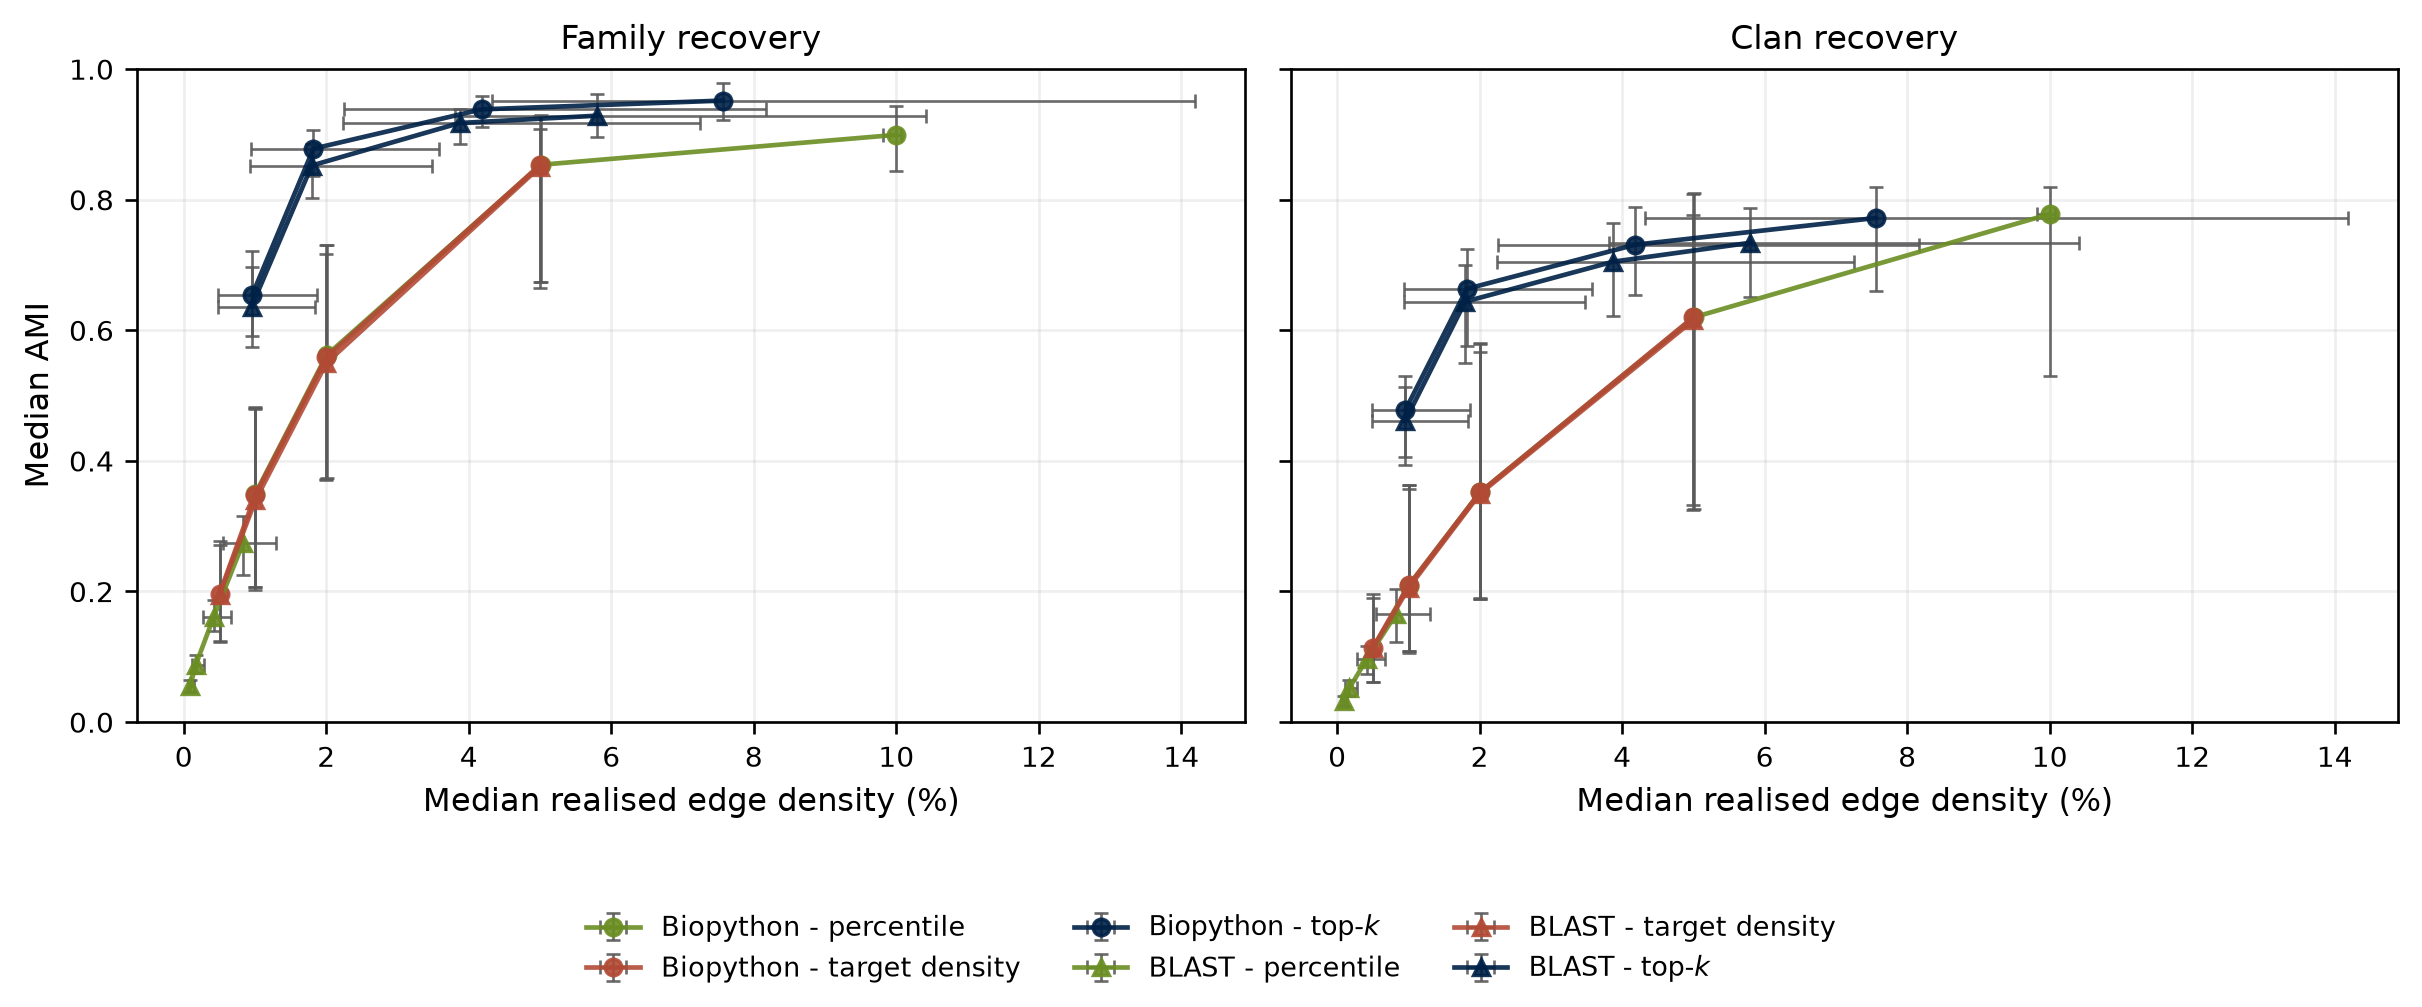
\includegraphics[width=\textwidth]{rule_recovery.png}
  \caption{Median AMI against median realised density across
  \PrimaryCollections\ primary collections. Panels show family and clan
  recovery. Lines connect parameter values within each method and rule family.
  Error bars give interquartile ranges across collections in both coordinates.
  Marker denotes score method: circle for Biopython, triangle for BLAST.}
  \label{fig:rules}
\end{figure}

Figure~\ref{fig:representative} shows one reference-condition top-5 example.
Each panel contains \RepresentativeNodes\ vertices from
\RepresentativeFamilies\ families. Biopython retained
\RepresentativeBioEdges\ edges in \RepresentativeBioComponents\ connected
components; BLAST retained \RepresentativeBlastEdges\ edges in
\RepresentativeBlastComponents\ components. Both family AMI values round to
\RepresentativeBioAMI, although component structures differ.

Each vertex represents one domain; colour denotes withheld Pfam family. Each
island is a connected component. Components are packed into a grid, then
vertices within each component receive a spring layout. Shared coordinates
permit vertex-wise comparison between panels; distance between islands carries
no analytical meaning.

\begin{figure}[!t]
  \centering
  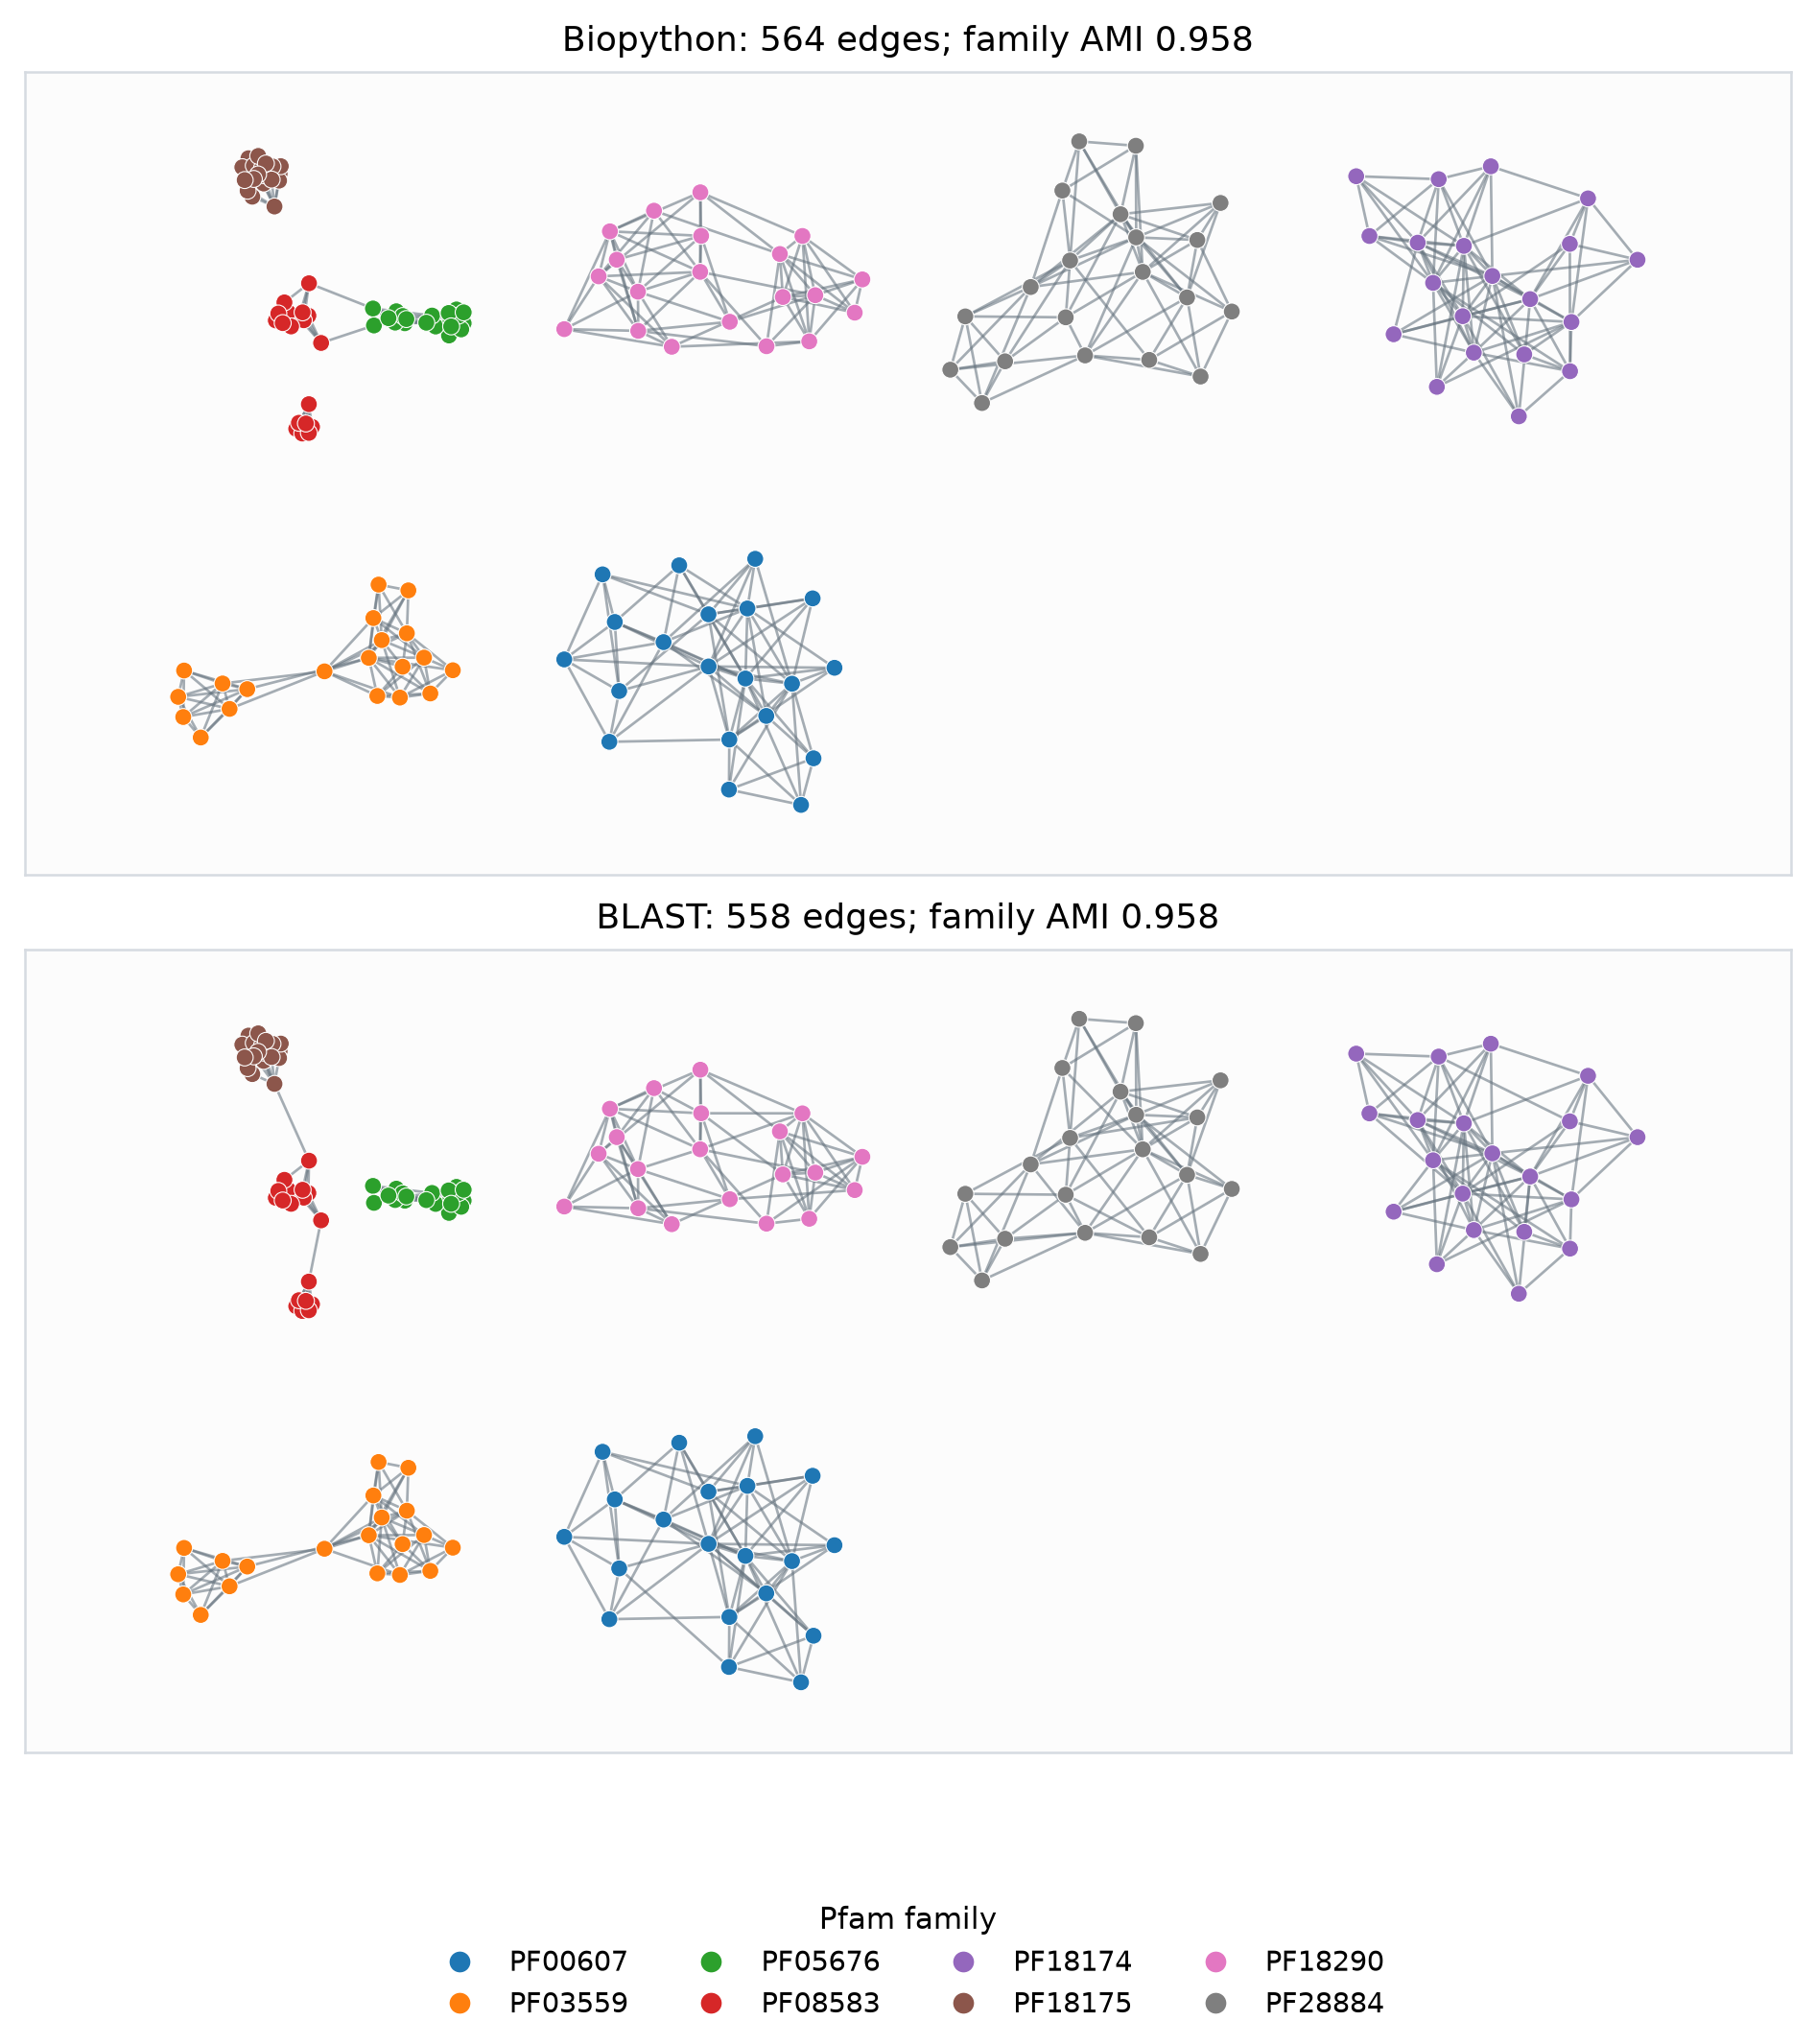
\includegraphics[width=0.90\textwidth]{representative_graphs.png}
  \caption{Biopython and BLAST top-5 graphs for collection
  \texttt{c4\_f2\_d20\_r001}. Colour denotes withheld Pfam family; islands are
  connected components. Panels share coordinates.}
  \label{fig:representative}
\end{figure}

\subsection{Effect of sparsity on structure recovery}
\label{sec:sparsity}

Realised density \(\delta=\lvert E\rvert/P\) reads directly as an edge
fraction, so \(\delta=0.04\) means 4\% of possible pairs are edges. Target
density falls short of its request whenever
\(\lvert A_m\rvert<\lceil dP\rceil\).

Reference composition fixes vertex count and family mixture. Within this
condition, connected-component and Louvain-community counts fell as realised
density increased (Fig.~\ref{fig:rule-topology}). At similar density, top-\(k\)
graphs contained fewer components than percentile and target-density graphs.
Top-\(k\) allocates local neighbours to every vertex; global rules can
concentrate edges among a subset of vertices. Fragmentation split Pfam groups
across many inferred communities and reduced AMI.

\begin{figure}[htbp]
  \centering
  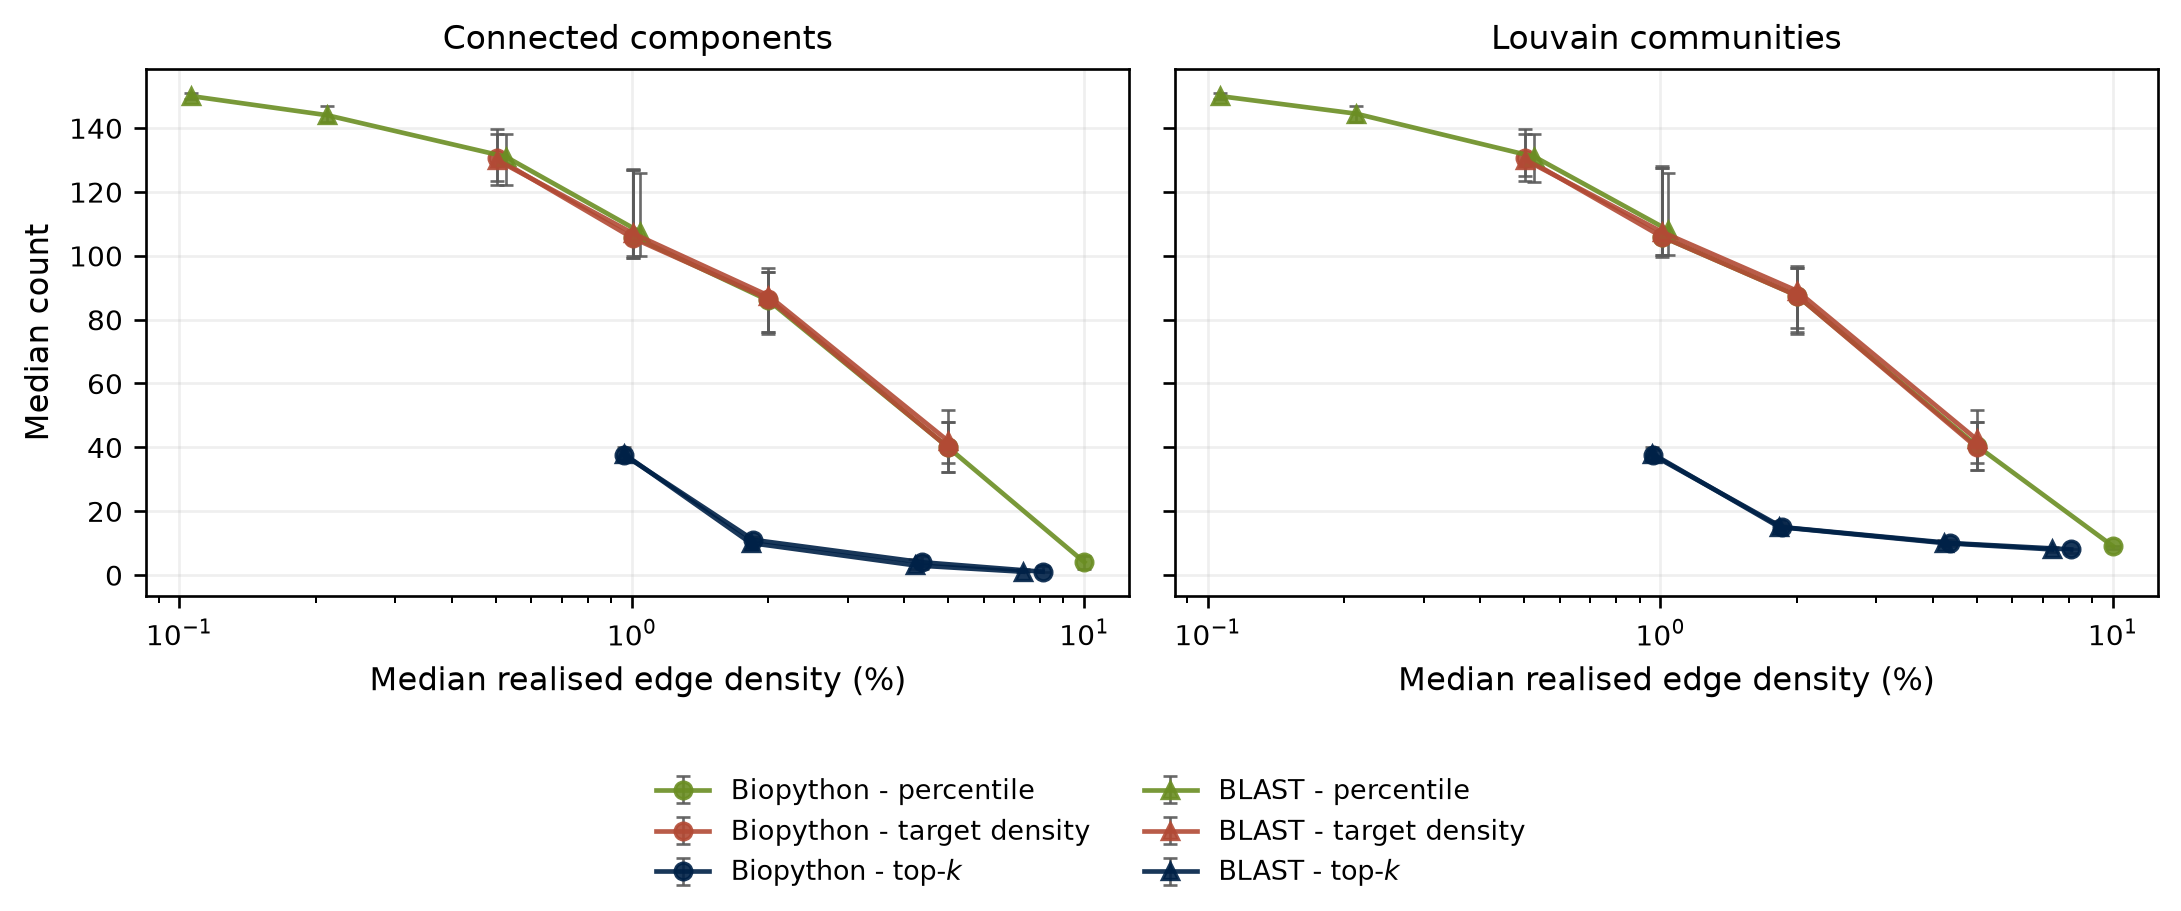
\includegraphics[width=\textwidth]{rule_topology.png}
  \caption{Median component and community counts against realised density for
  12 graph settings and \ReplicatesPerCondition\ reference-condition
  collections. Colour denotes rule family; marker denotes score method, circle
  for Biopython and triangle for BLAST. Error bars give interquartile ranges
  across collections.}
  \label{fig:rule-topology}
\end{figure}

\subsection{AMI as primary agreement measure}

NMI and AMI agreed for dense graphs whose inferred community counts approached
reference group counts (Fig.~\ref{fig:metric-comparison}). Their difference
grew under sparse percentile and target-density rules. For BLAST percentile
0.99, median partition contained \BlastPercentileNinetyNineCommunities\
communities for 8 reference families. Median family NMI was
\BlastPercentileNinetyNineNMI; median AMI was
\BlastPercentileNinetyNineAMI. NMI retained agreement produced by many small
groups, while AMI subtracted expected agreement conditional on group sizes.

\begin{figure}[htbp]
  \centering
  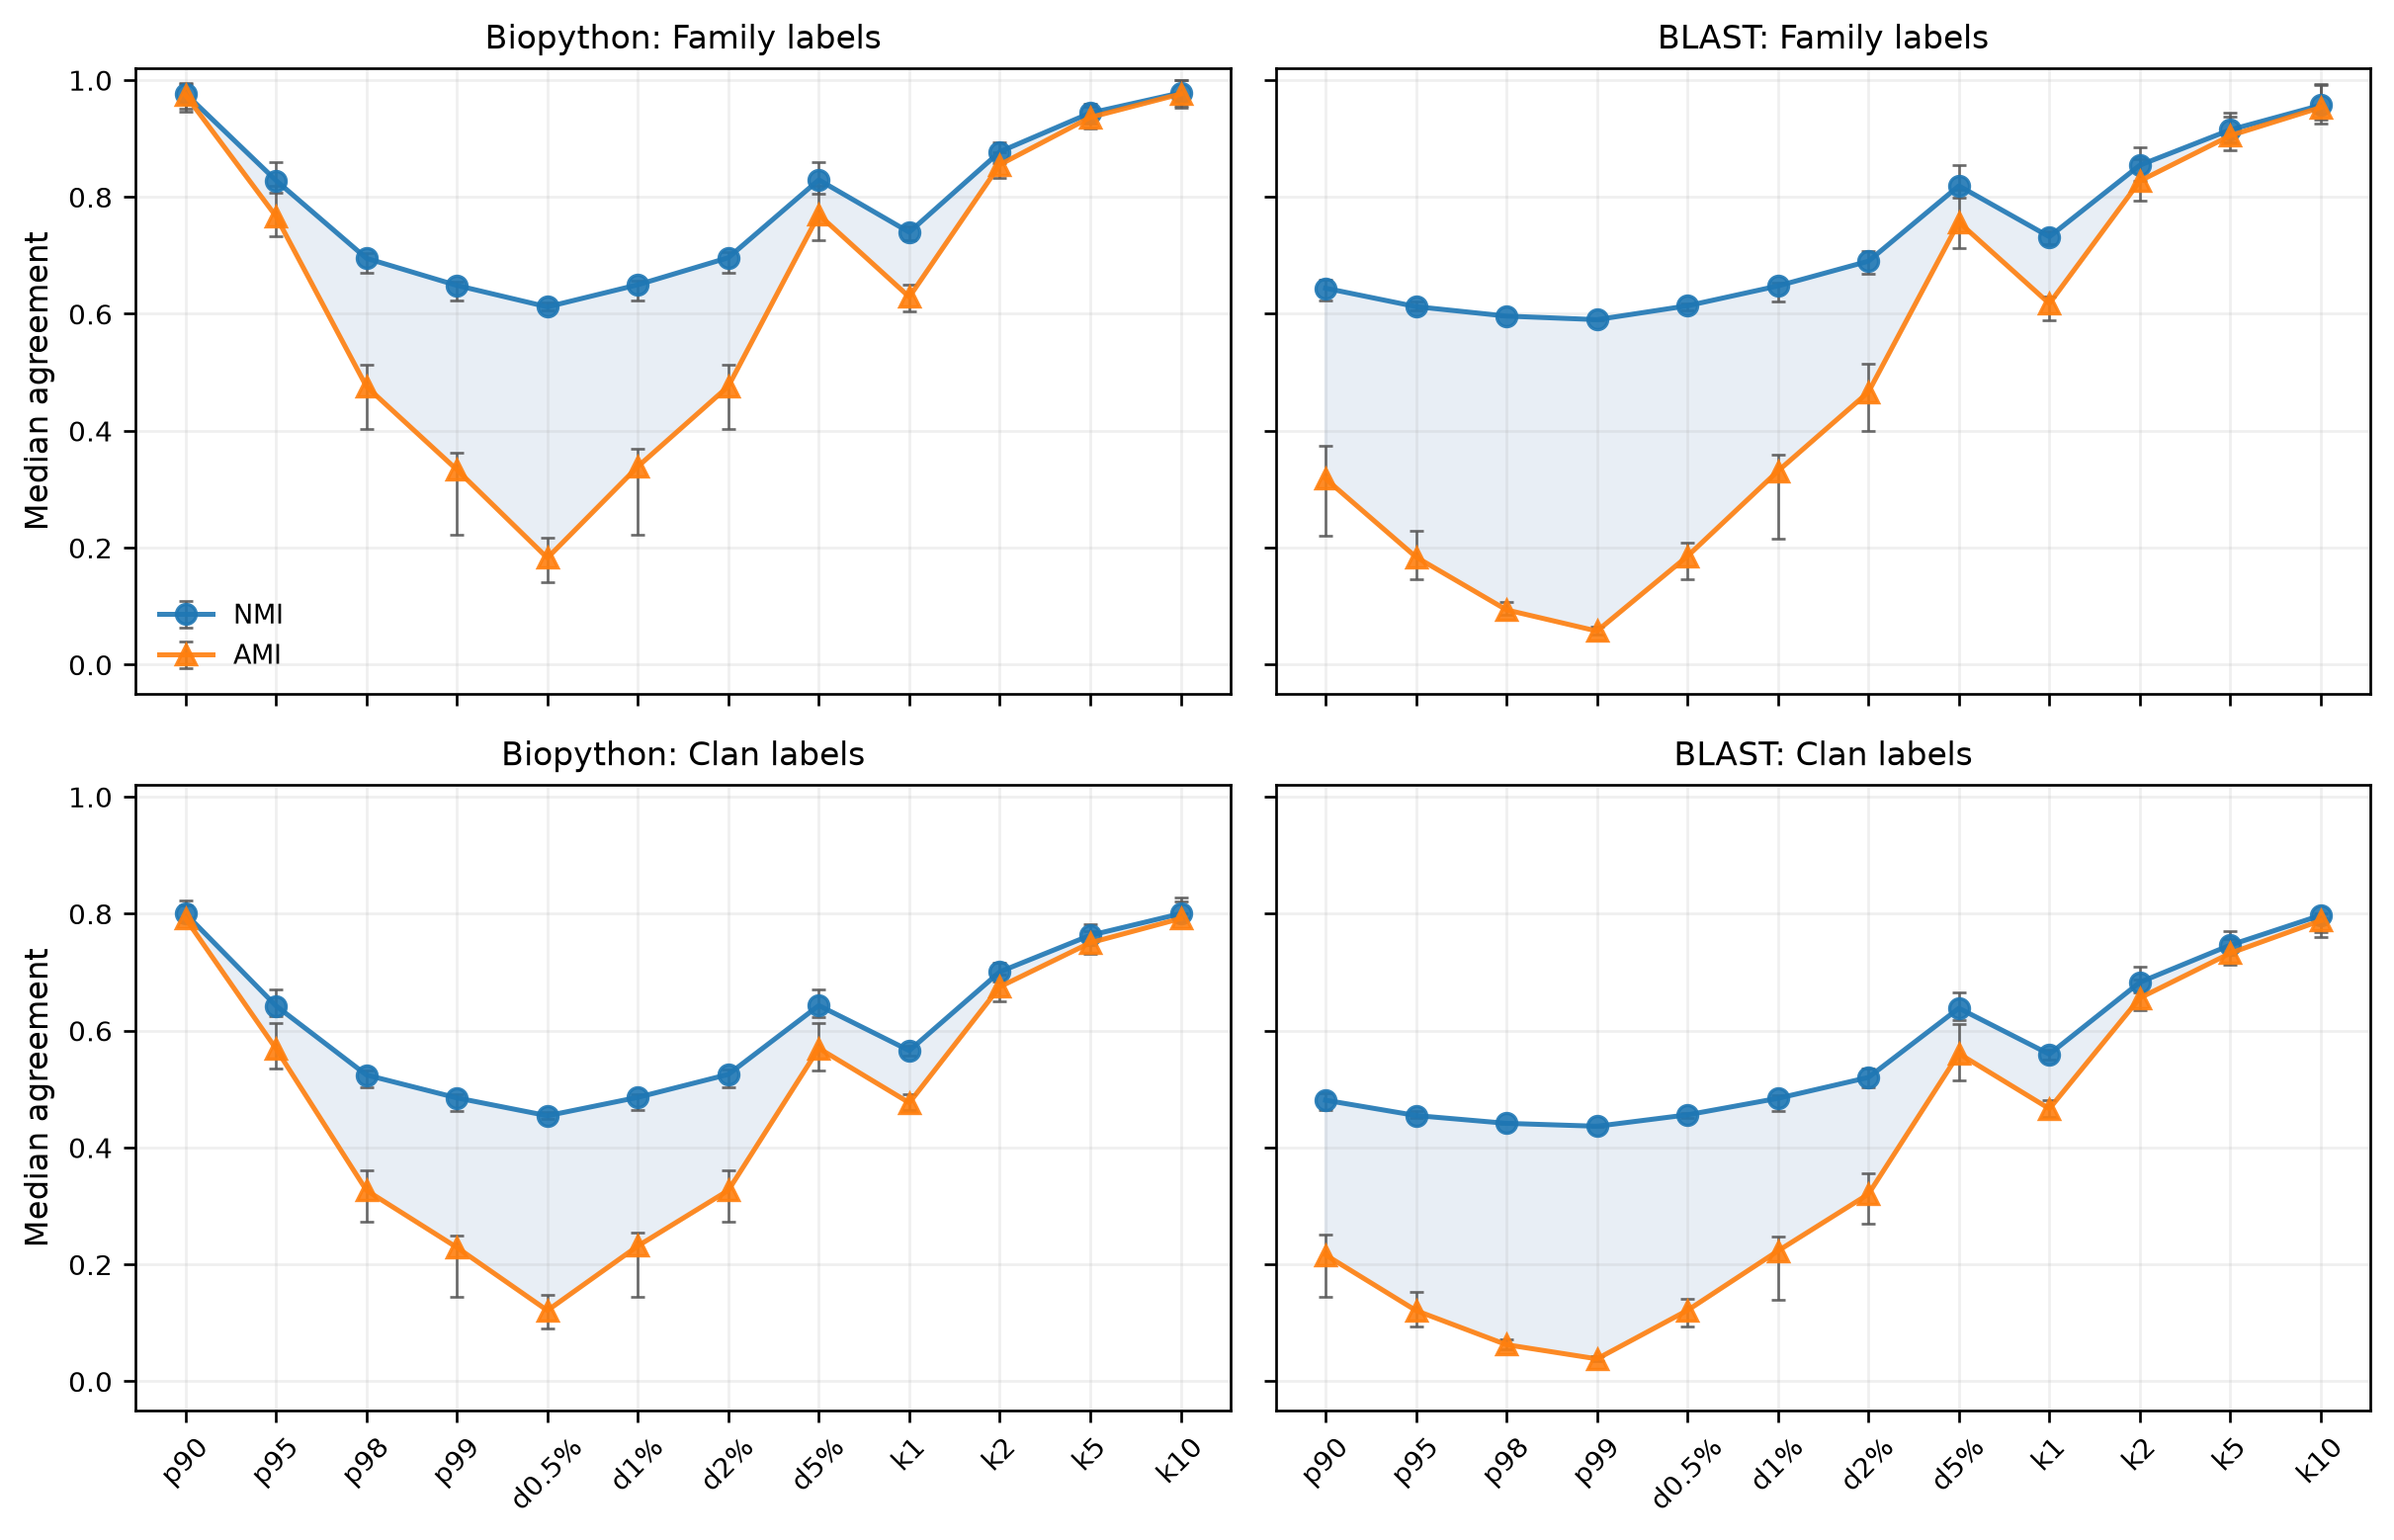
\includegraphics[width=\textwidth]{metric_comparison.png}
  \caption{Median NMI and AMI for 12 graph settings in reference condition,
  with interquartile ranges across collections as error bars.
  Panels separate score method and withheld label level. Shading marks chance
  correction. Prefixes \(p\), \(d\), and \(k\) denote percentile, target
  density, and top-\(k\).}
  \label{fig:metric-comparison}
\end{figure}

Figures~\ref{fig:nmi-frequency} and~\ref{fig:ami-frequency} show frequency
polygons derived from replicate distributions behind
Fig.~\ref{fig:metric-comparison}. Each of
\ReplicatesPerCondition\ collections contributes one graph to every
score-method and graph-setting combination. Agreement values are placed in 25
equal-width bins on \([0,1]\). Vertical position gives percentage of collection
graphs in each bin; frequencies for each curve sum to 100\%. AMI moved sparse-rule
distributions towards zero. Primary rule comparisons therefore use AMI; NMI
remains a bounded description of unadjusted partition agreement.

\begin{figure}[htbp]
  \centering
  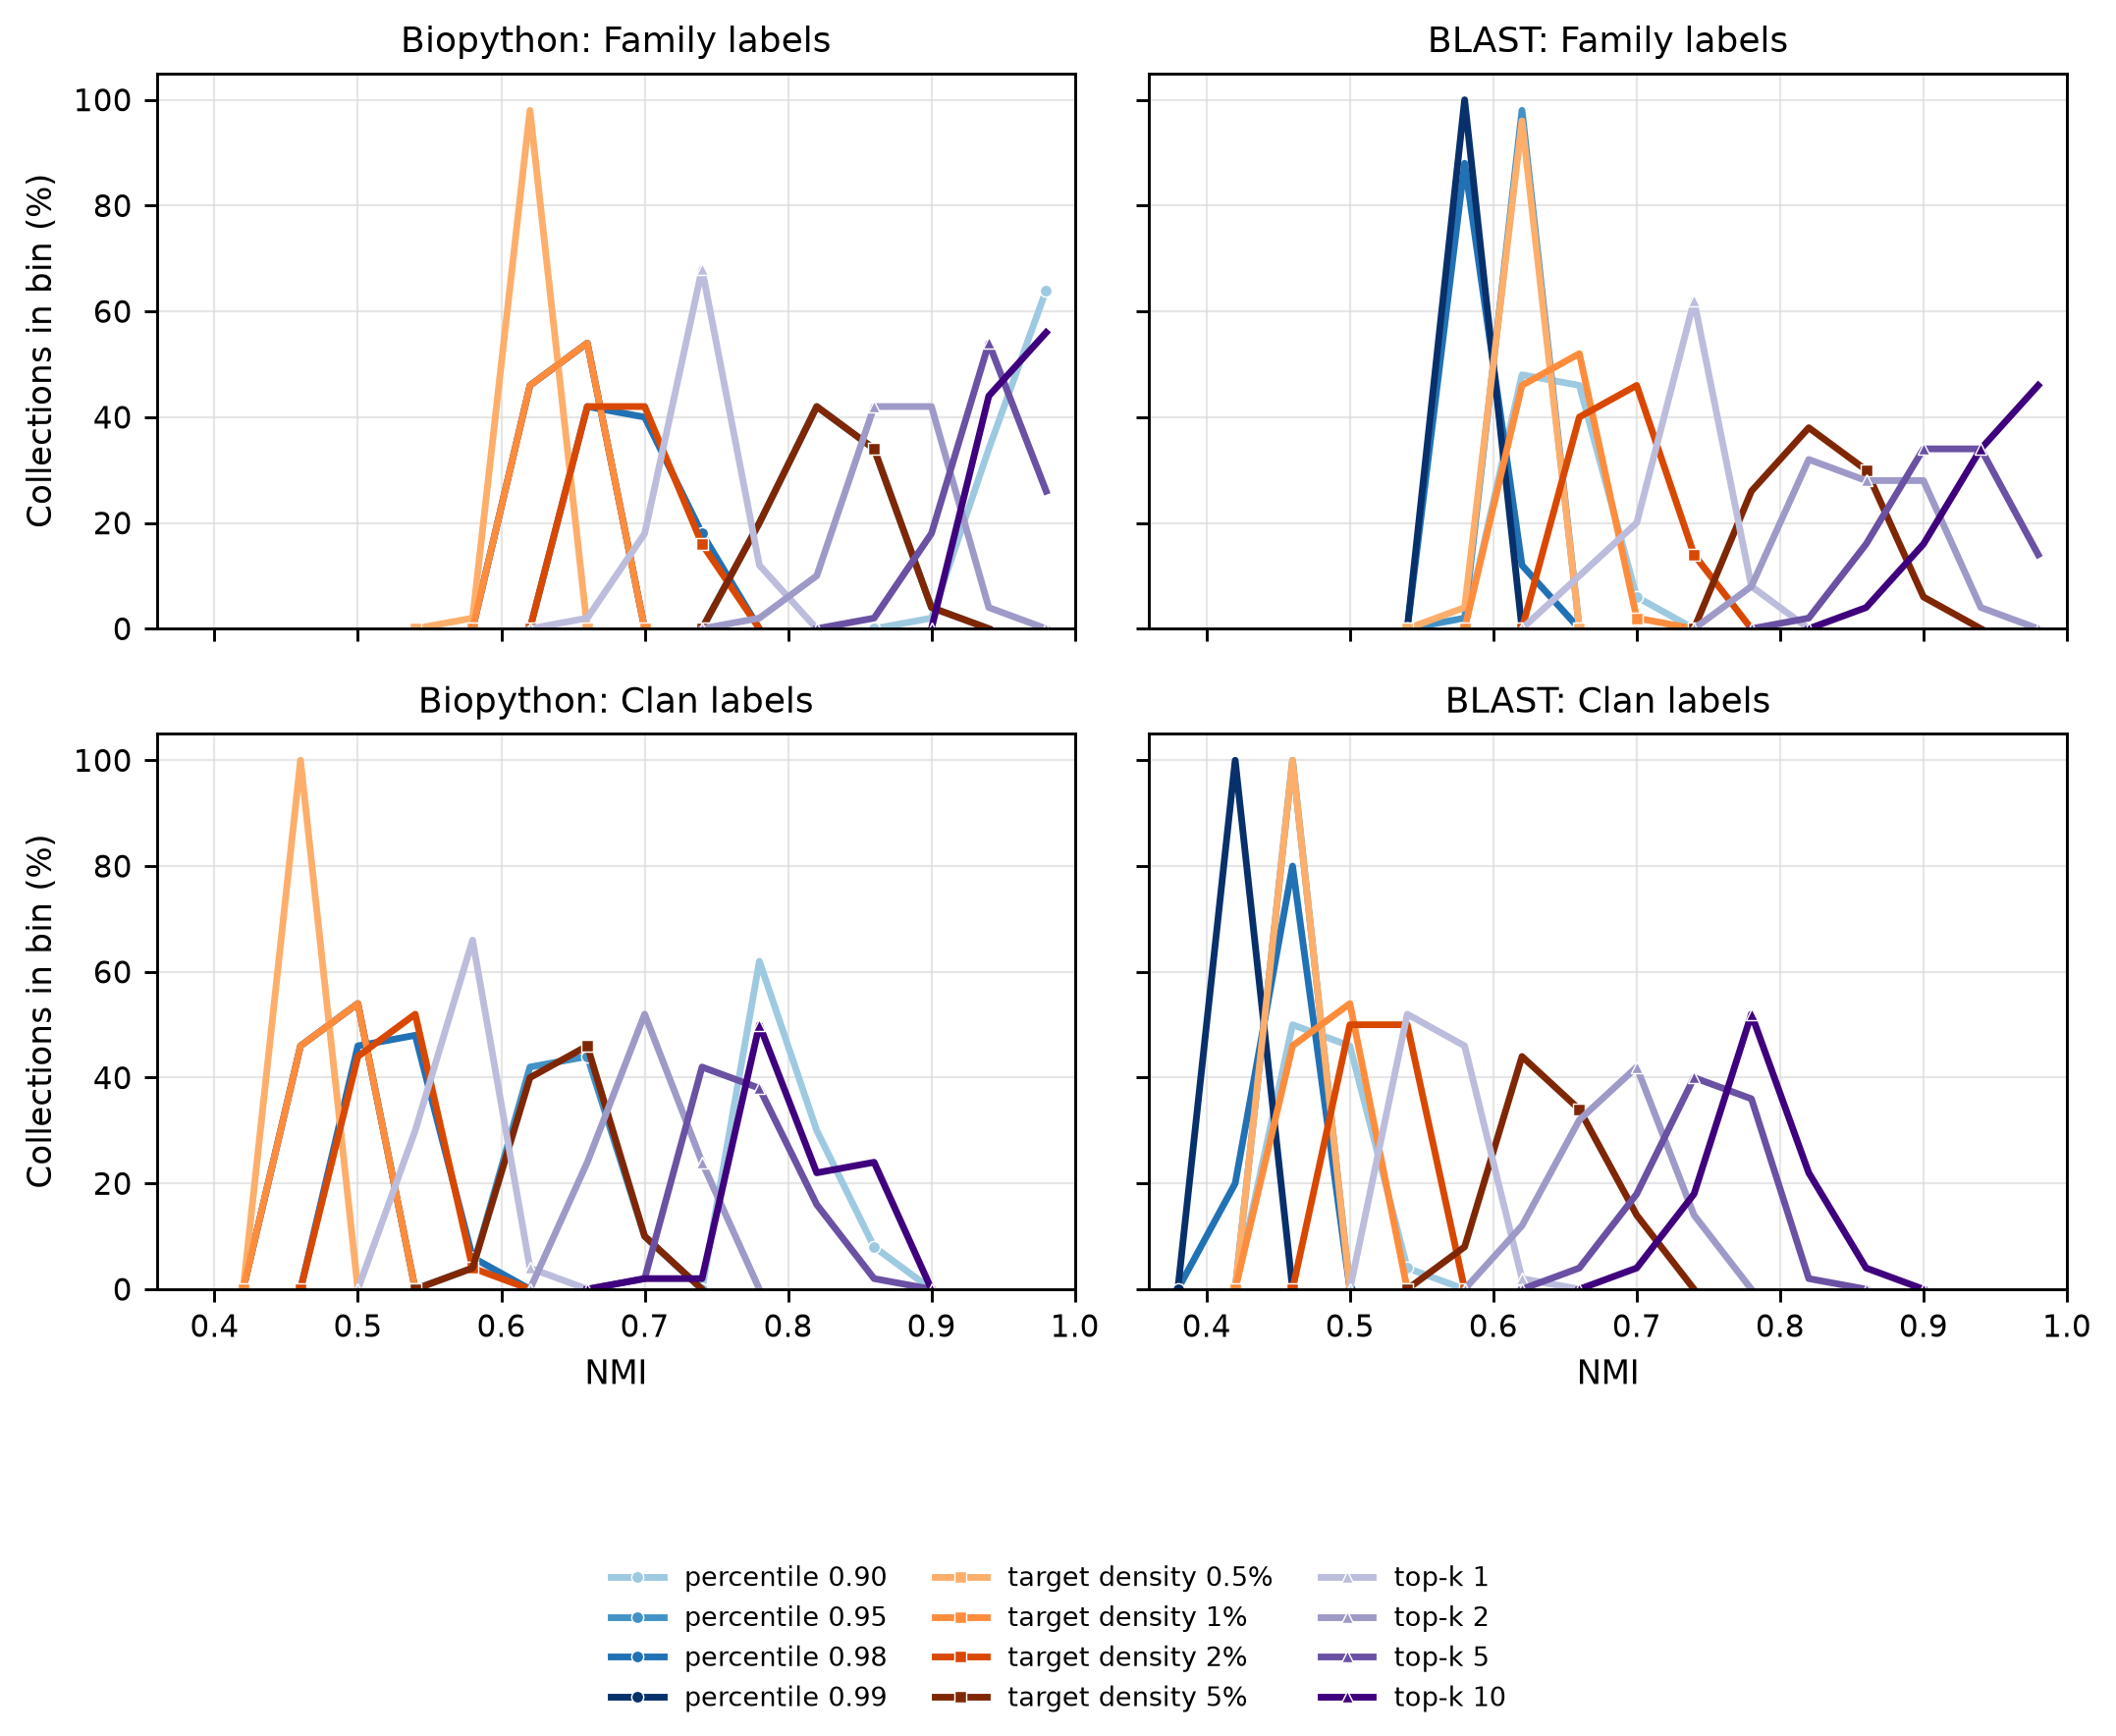
\includegraphics[width=0.88\textwidth]{rule_nmi_frequency.png}
  \caption{Empirical NMI frequency polygons across 12 graph settings and
  \ReplicatesPerCondition\ reference-condition collections. Each curve joins
  percentages of collection graphs in 25 equal-width NMI bins. Panels separate
  score method and withheld label level. Line style and marker denote rule
  family; colour distinguishes parameter values within each family.}
  \label{fig:nmi-frequency}
\end{figure}

\begin{figure}[htbp]
  \centering
  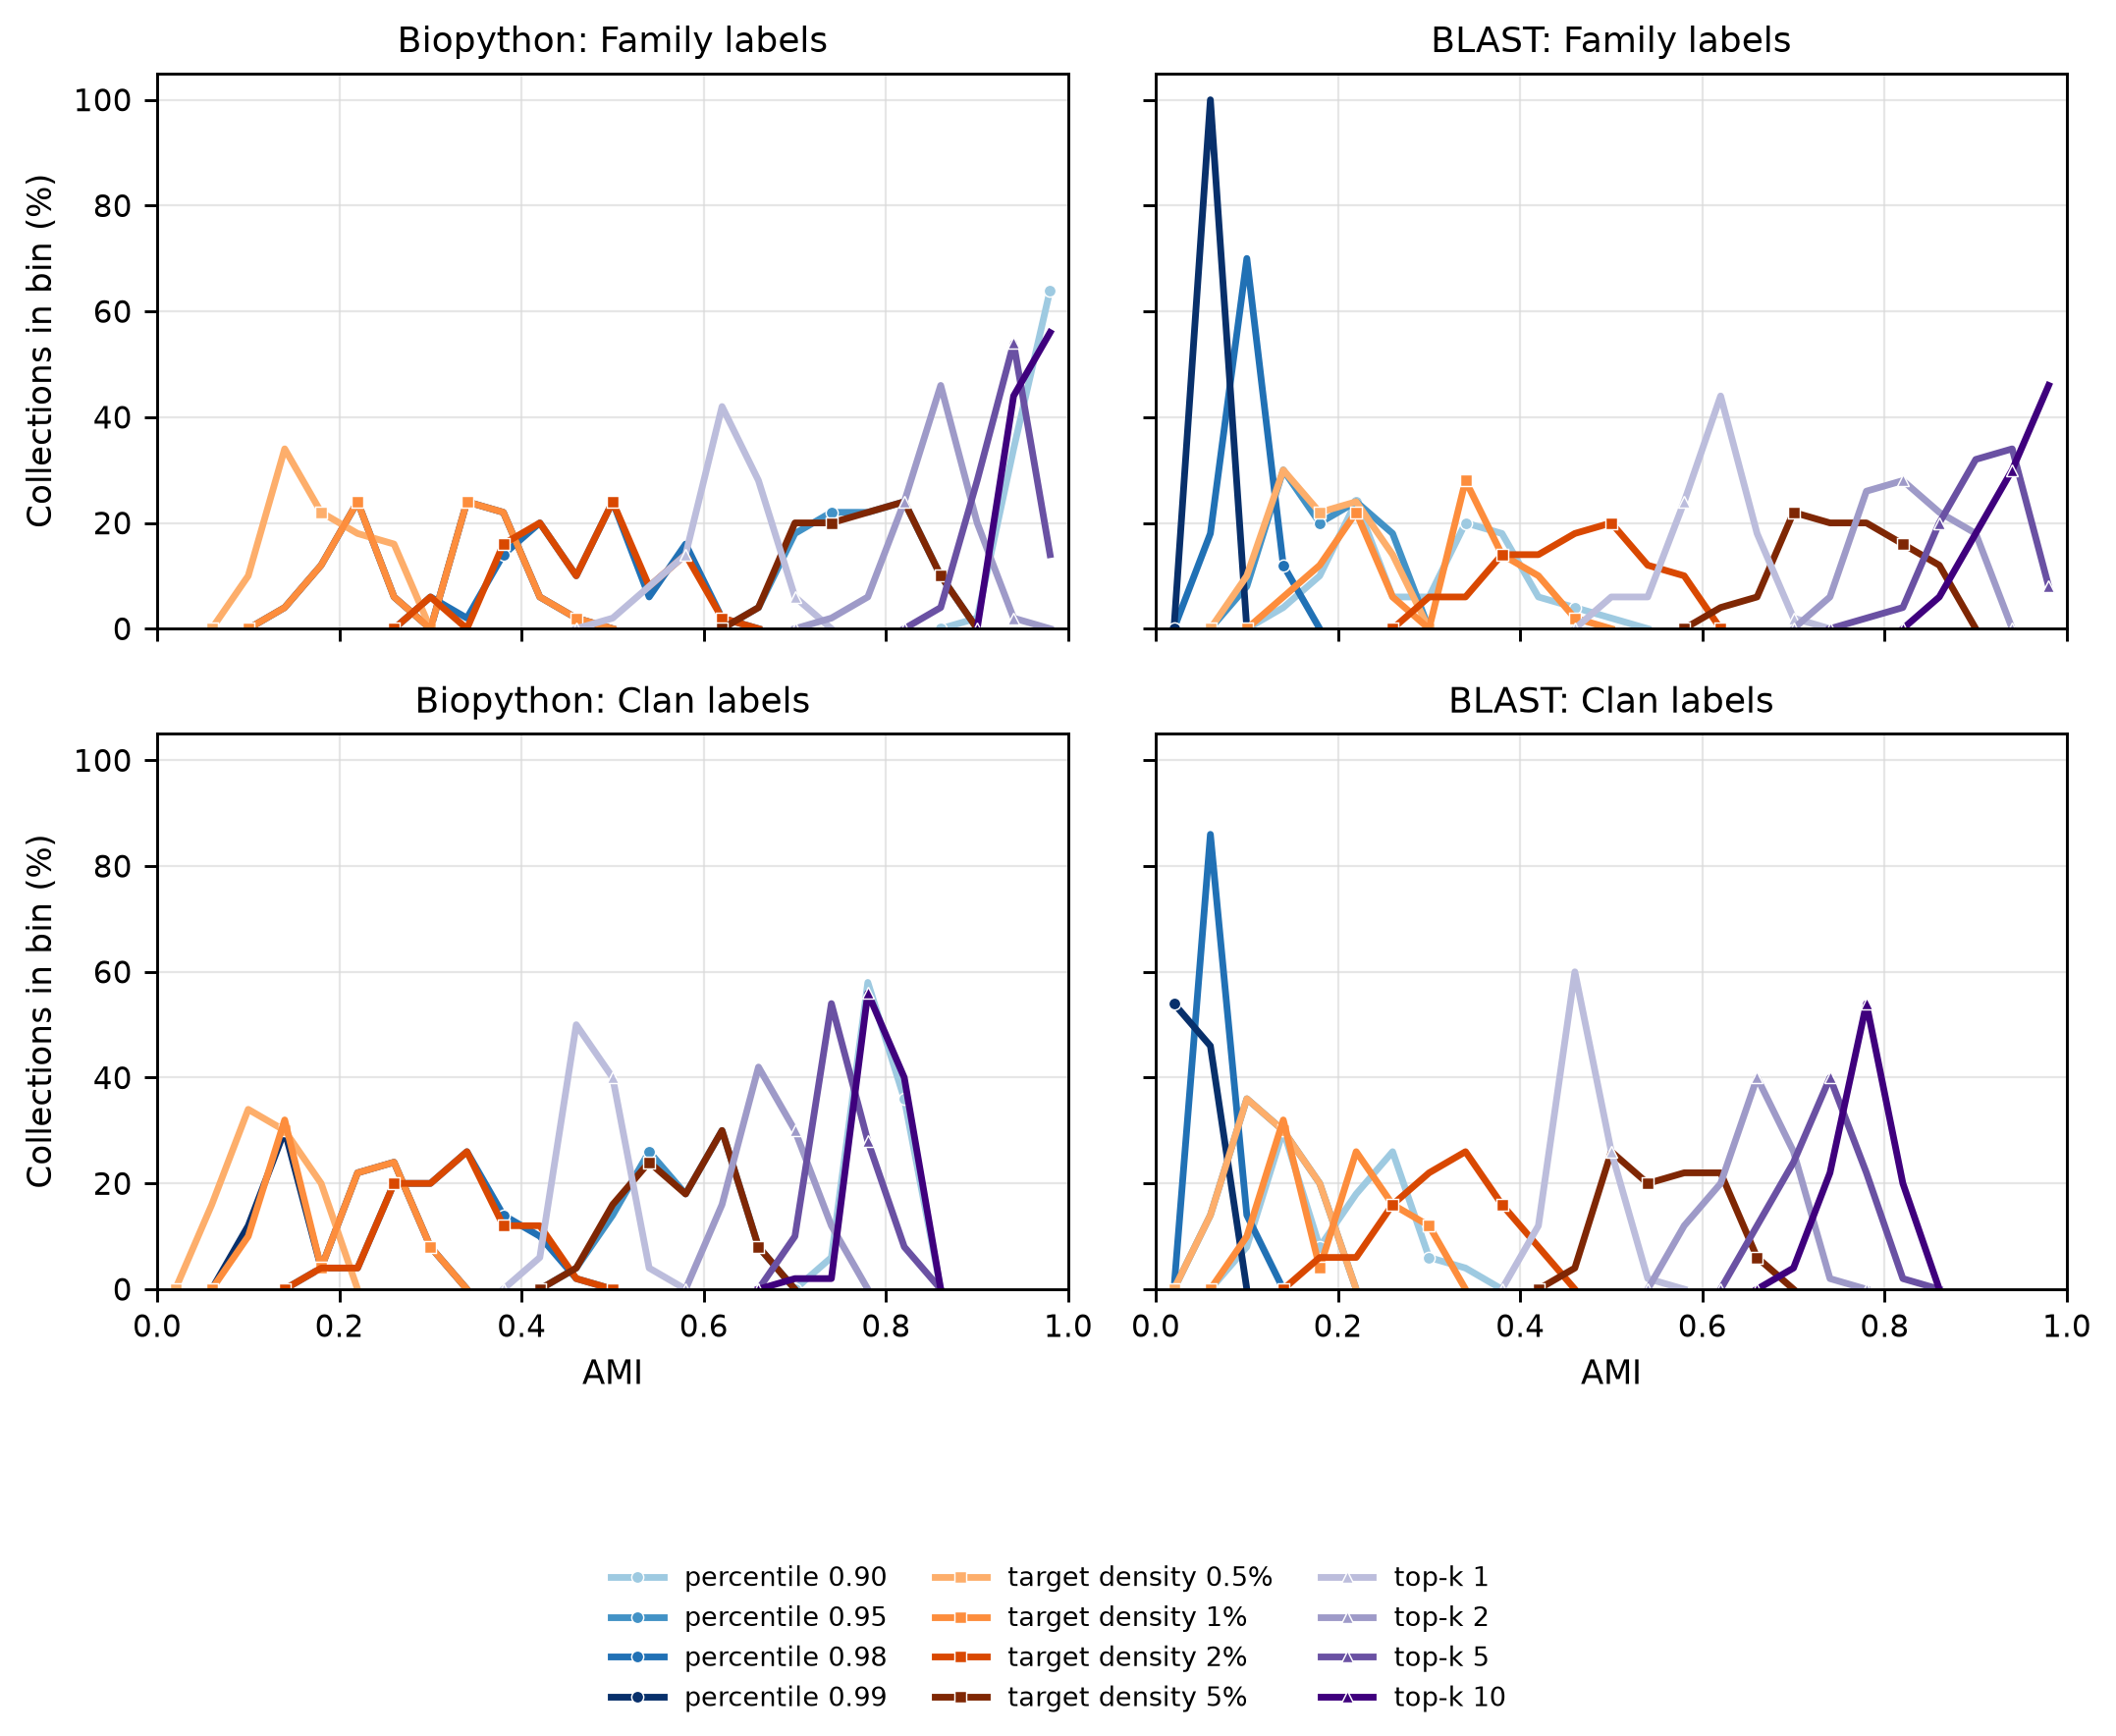
\includegraphics[width=0.88\textwidth]{rule_ami_frequency.png}
  \caption{Empirical AMI frequency polygons for graphs in
  Fig.~\ref{fig:nmi-frequency}. Panels, curves, bins, and visual encodings follow
  same design.}
  \label{fig:ami-frequency}
\end{figure}

\subsection{Effect of score method on graph-rule conclusions}
\label{sec:percentile}

Top-\(k\) led family recovery under both score methods
(Fig.~\ref{fig:rules}). Biopython scored all \MasterPairs\ master-panel pairs;
BLAST reported \BlastReportedPairs\ pairs, or \BlastCoveragePct\%. Among
reported pairs, score ranks had Spearman correlation \SharedScoreSpearman\
(Fig.~\ref{fig:score-coverage}, left). BLAST reports concentrated among pairs
with high Biopython scores (Fig.~\ref{fig:score-coverage}, right).

\begin{figure}[htbp]
  \centering
  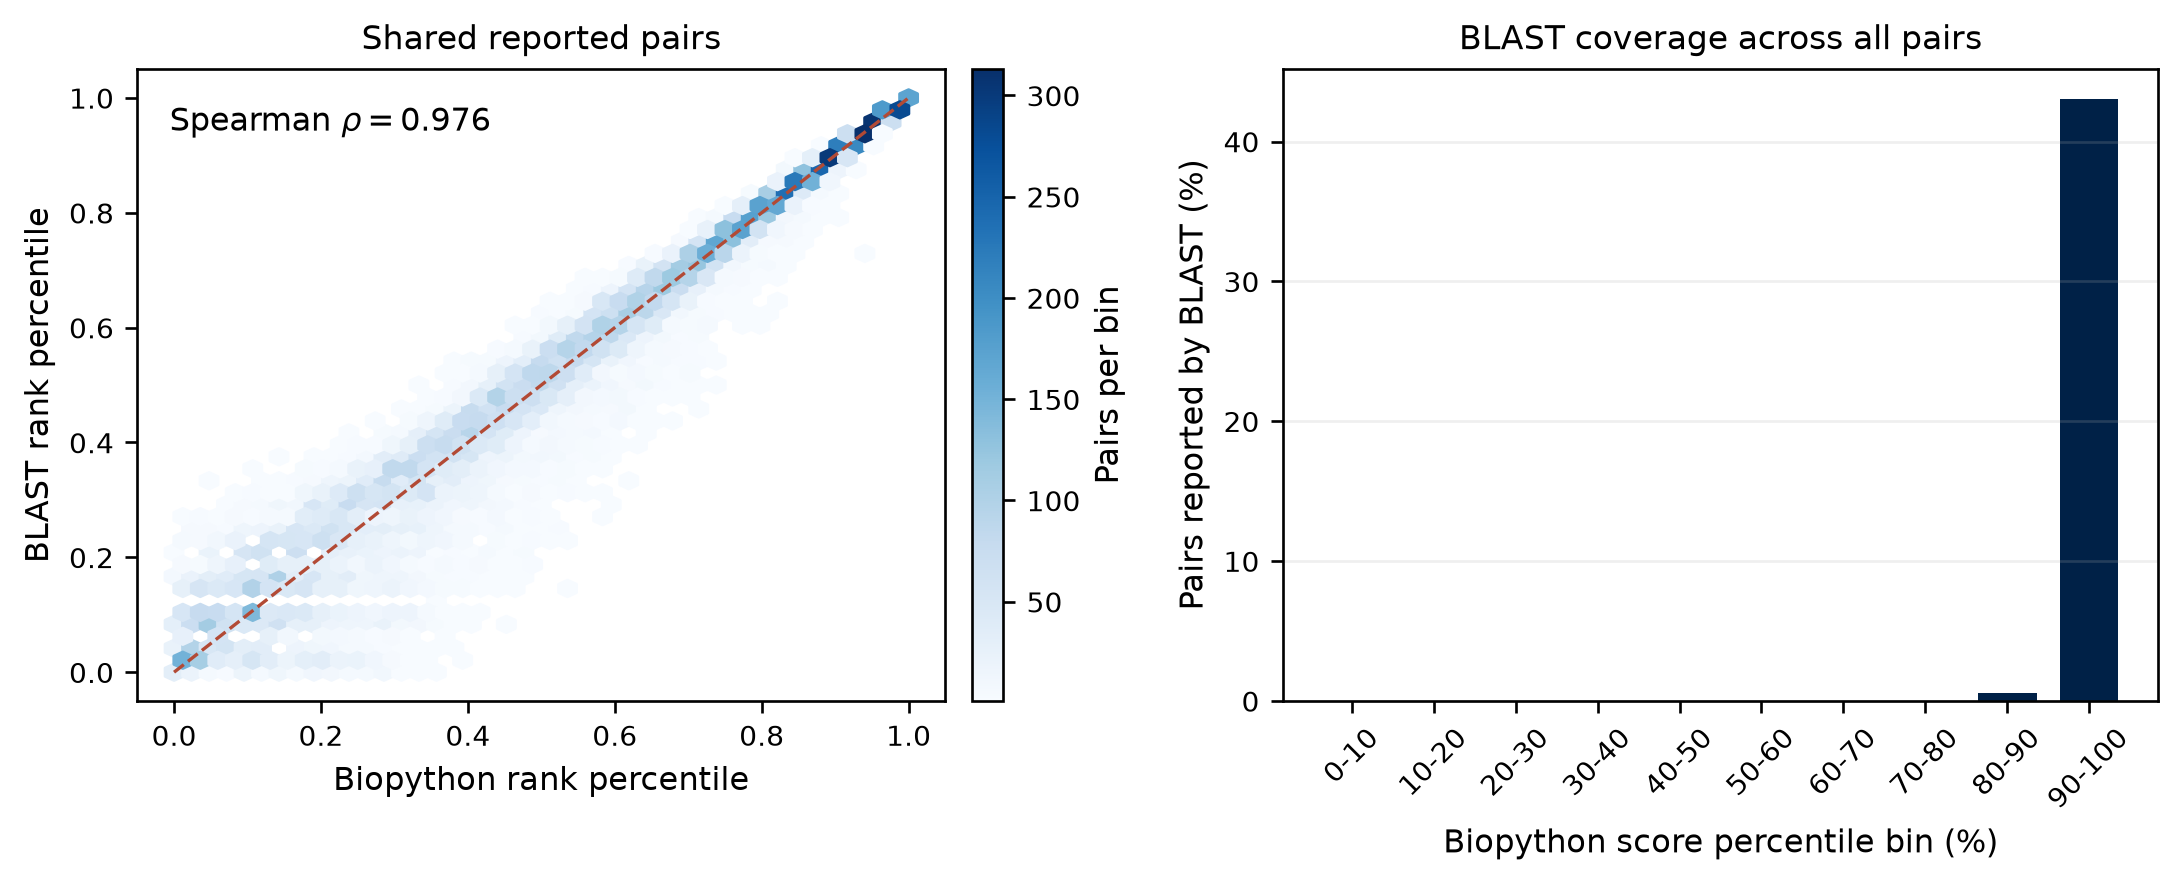
\includegraphics[width=\textwidth]{score_method_comparison.png}
  \caption{Pair-score comparison on master panel. Left: within-method rank
  percentiles among \BlastReportedPairs\ pairs reported by BLAST; colour gives
  bin count. Right: fraction reported by BLAST within each Biopython score
  percentile bin across all \MasterPairs\ pairs.}
  \label{fig:score-coverage}
\end{figure}

Percentile rules retain a fraction of each method's available scores. At
percentile 0.90, the median realised density was
\BioPercentileNinetyDensityPct\% for Biopython and
\BlastPercentileNinetyDensityPct\% for BLAST
(Fig.~\ref{fig:percentile}). Equal percentile parameters therefore represented
different edge budgets.

\begin{figure}[htbp]
  \centering
  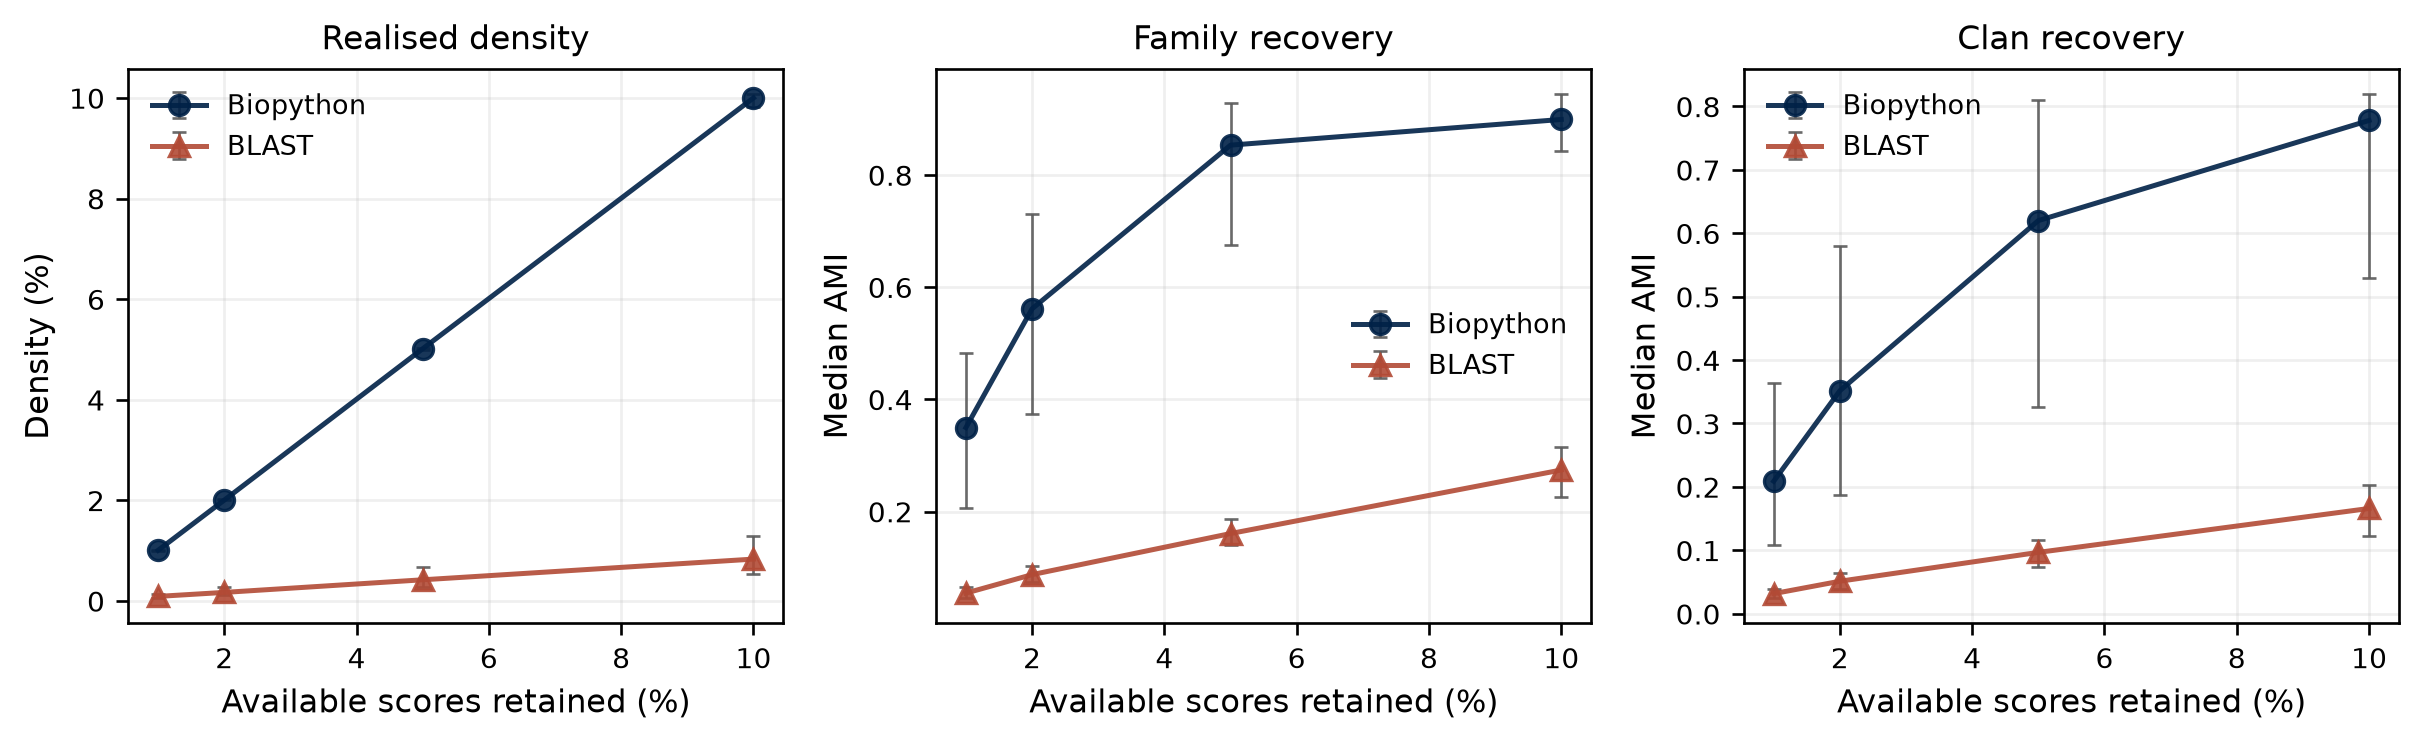
\includegraphics[width=\textwidth]{percentile_density_mismatch.png}
  \caption{Median density, family AMI, and clan AMI under percentile rules,
  with interquartile ranges across collections as error bars.
  Horizontal position is fraction of available scores retained within each
  method. Summaries use \PrimaryCollections\ primary collections.}
  \label{fig:percentile}
\end{figure}

Target density rules compare methods on identical vertex sets and requested
edge budgets. Budgets 0.5\%, 1\%, and 2\% were fully supplied, while a 5\%
request exceeded available BLAST pairs in some collections and was therefore
excluded from matched budget interpretation. At 2\%, paired median absolute
family difference was \MatchedTwoAbsDeltaNMI\ for NMI and
\MatchedTwoAbsDeltaAMI\ for AMI. Signed differences remained close to zero and
their spread increased with density (Fig.~\ref{fig:matched-density}).

\begin{figure}[htbp]
  \centering
  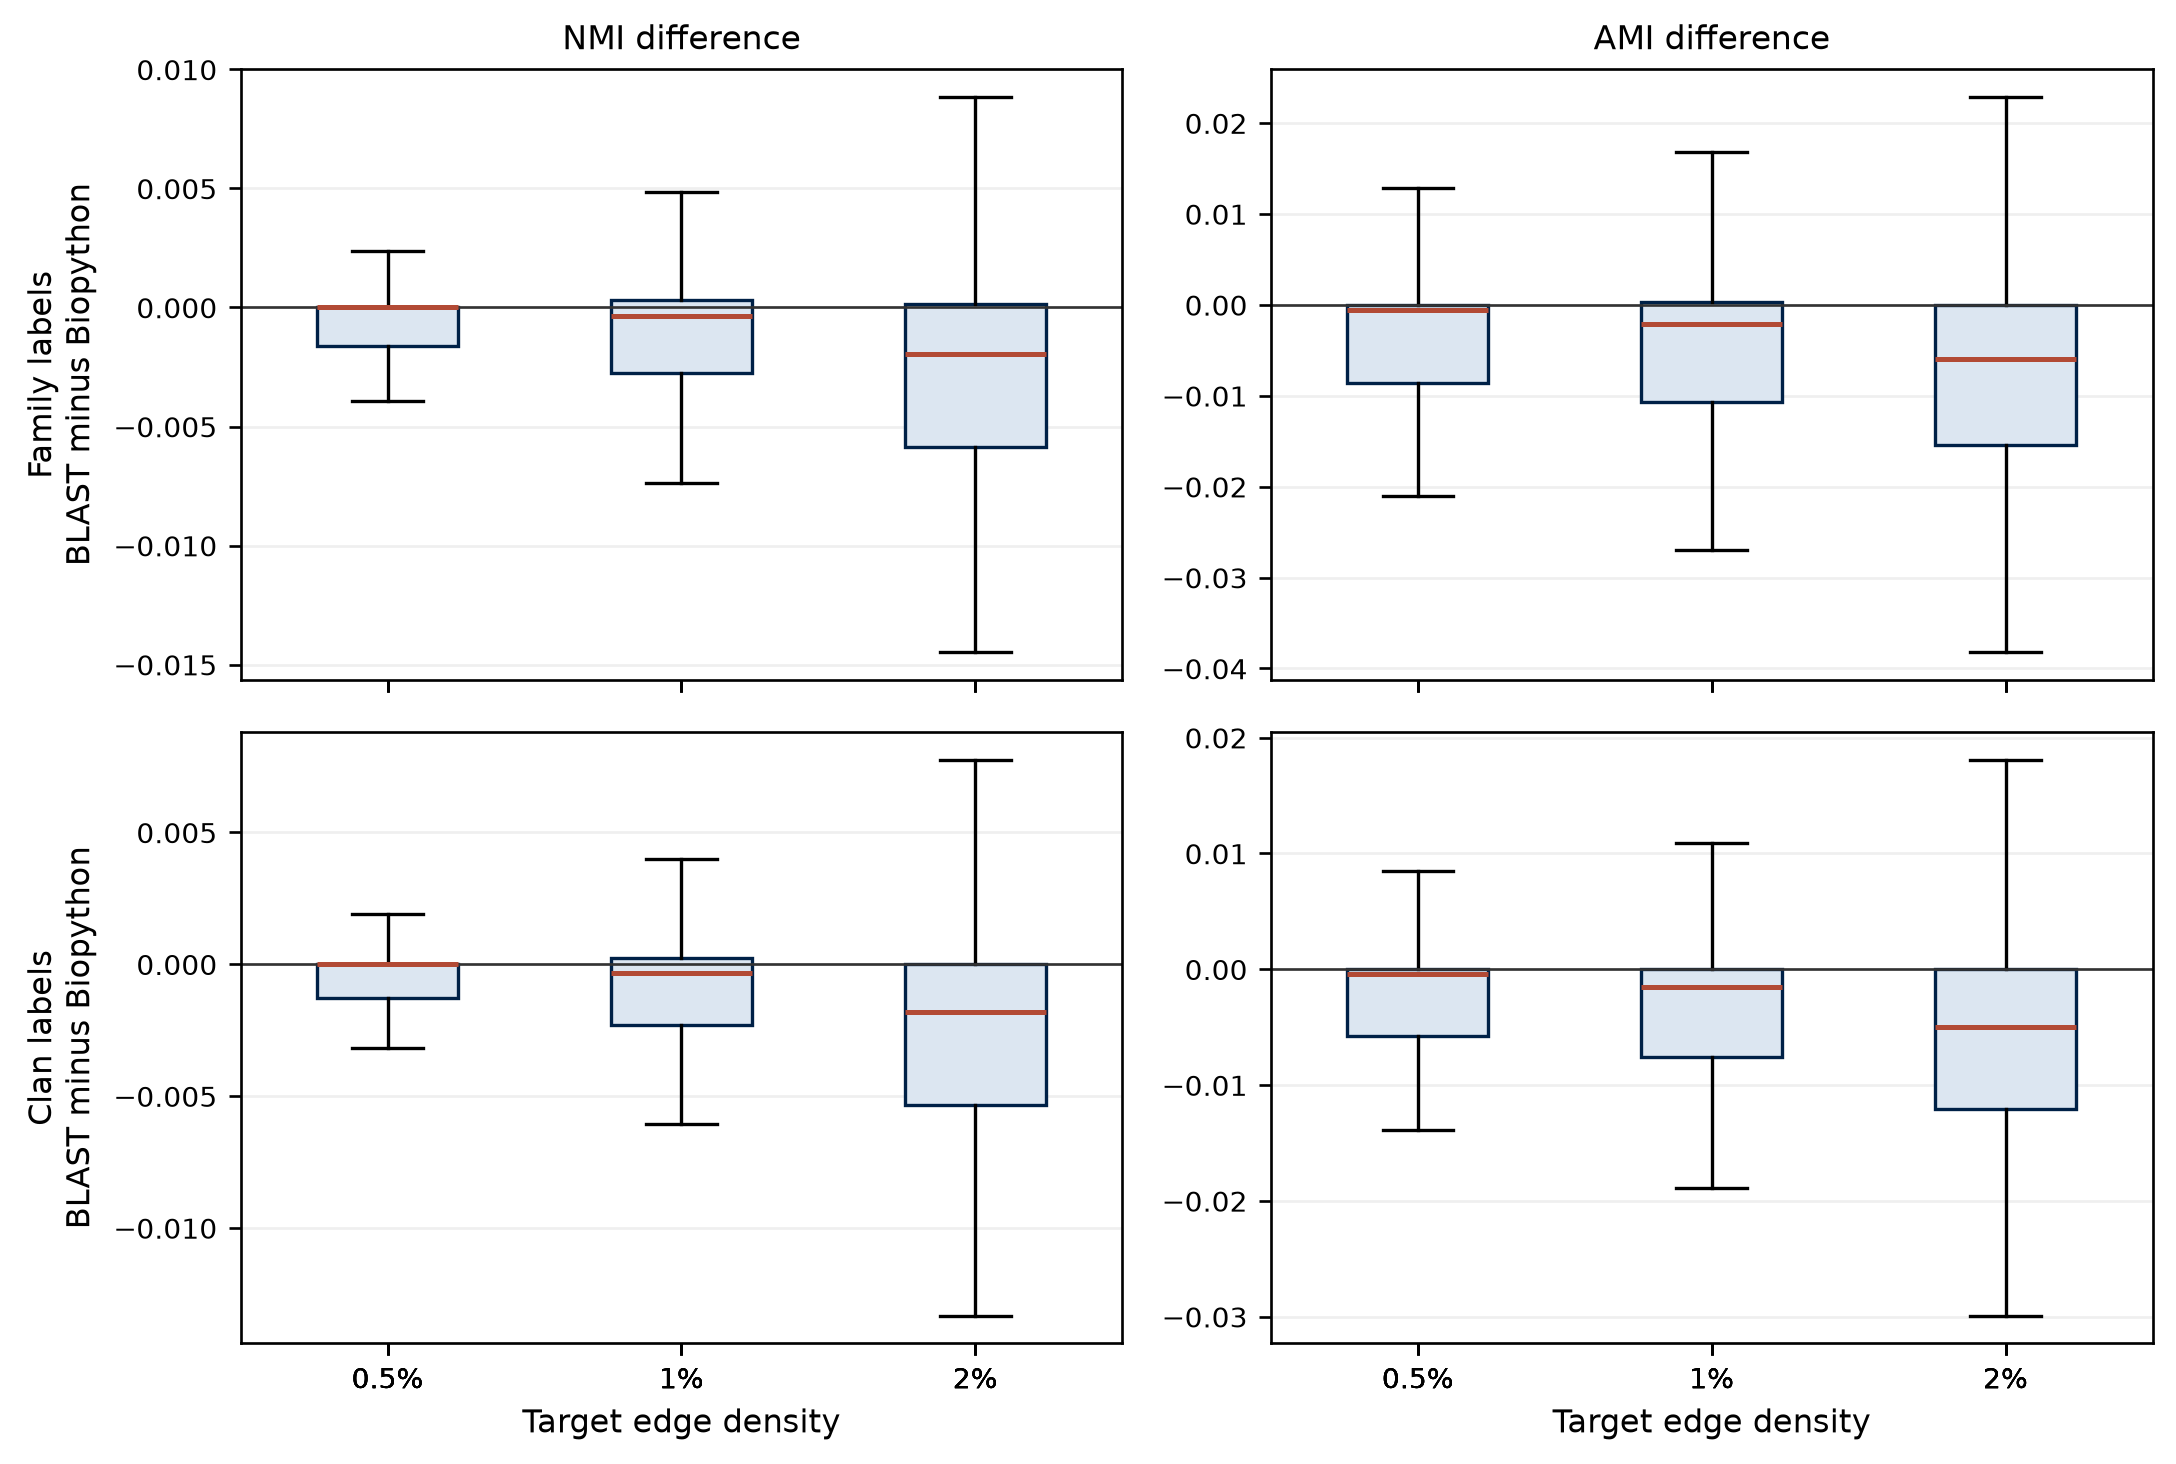
\includegraphics[width=\textwidth]{matched_density_differences.png}
  \caption{Paired NMI and AMI differences, BLAST minus Biopython, at matched
  edge densities across \PrimaryCollections\ collections. Boxes show
  quartiles and medians; whiskers extend to 1.5 interquartile ranges. Outliers
  are omitted from display.}%
  \label{fig:matched-density}
\end{figure}

\subsection{Effect of collection composition under a fixed rule}
\label{sec:composition}

Top-5 family AMI was evaluated across \PrimaryConditions\ primary composition
conditions, each with \ReplicatesPerCondition\ collections. Median family AMI
ranged from \CompositionMinAMI\ to \CompositionMaxAMI\ for Biopython and from
\BlastCompositionMinAMI\ to \BlastCompositionMaxAMI\ for BLAST
(Fig.~\ref{fig:composition}). Changes across domain, family, and clan counts
were non-monotone. Four saturated design cells remain in audit outputs and do
not enter these summaries.

\begin{figure}[htbp]
  \centering
  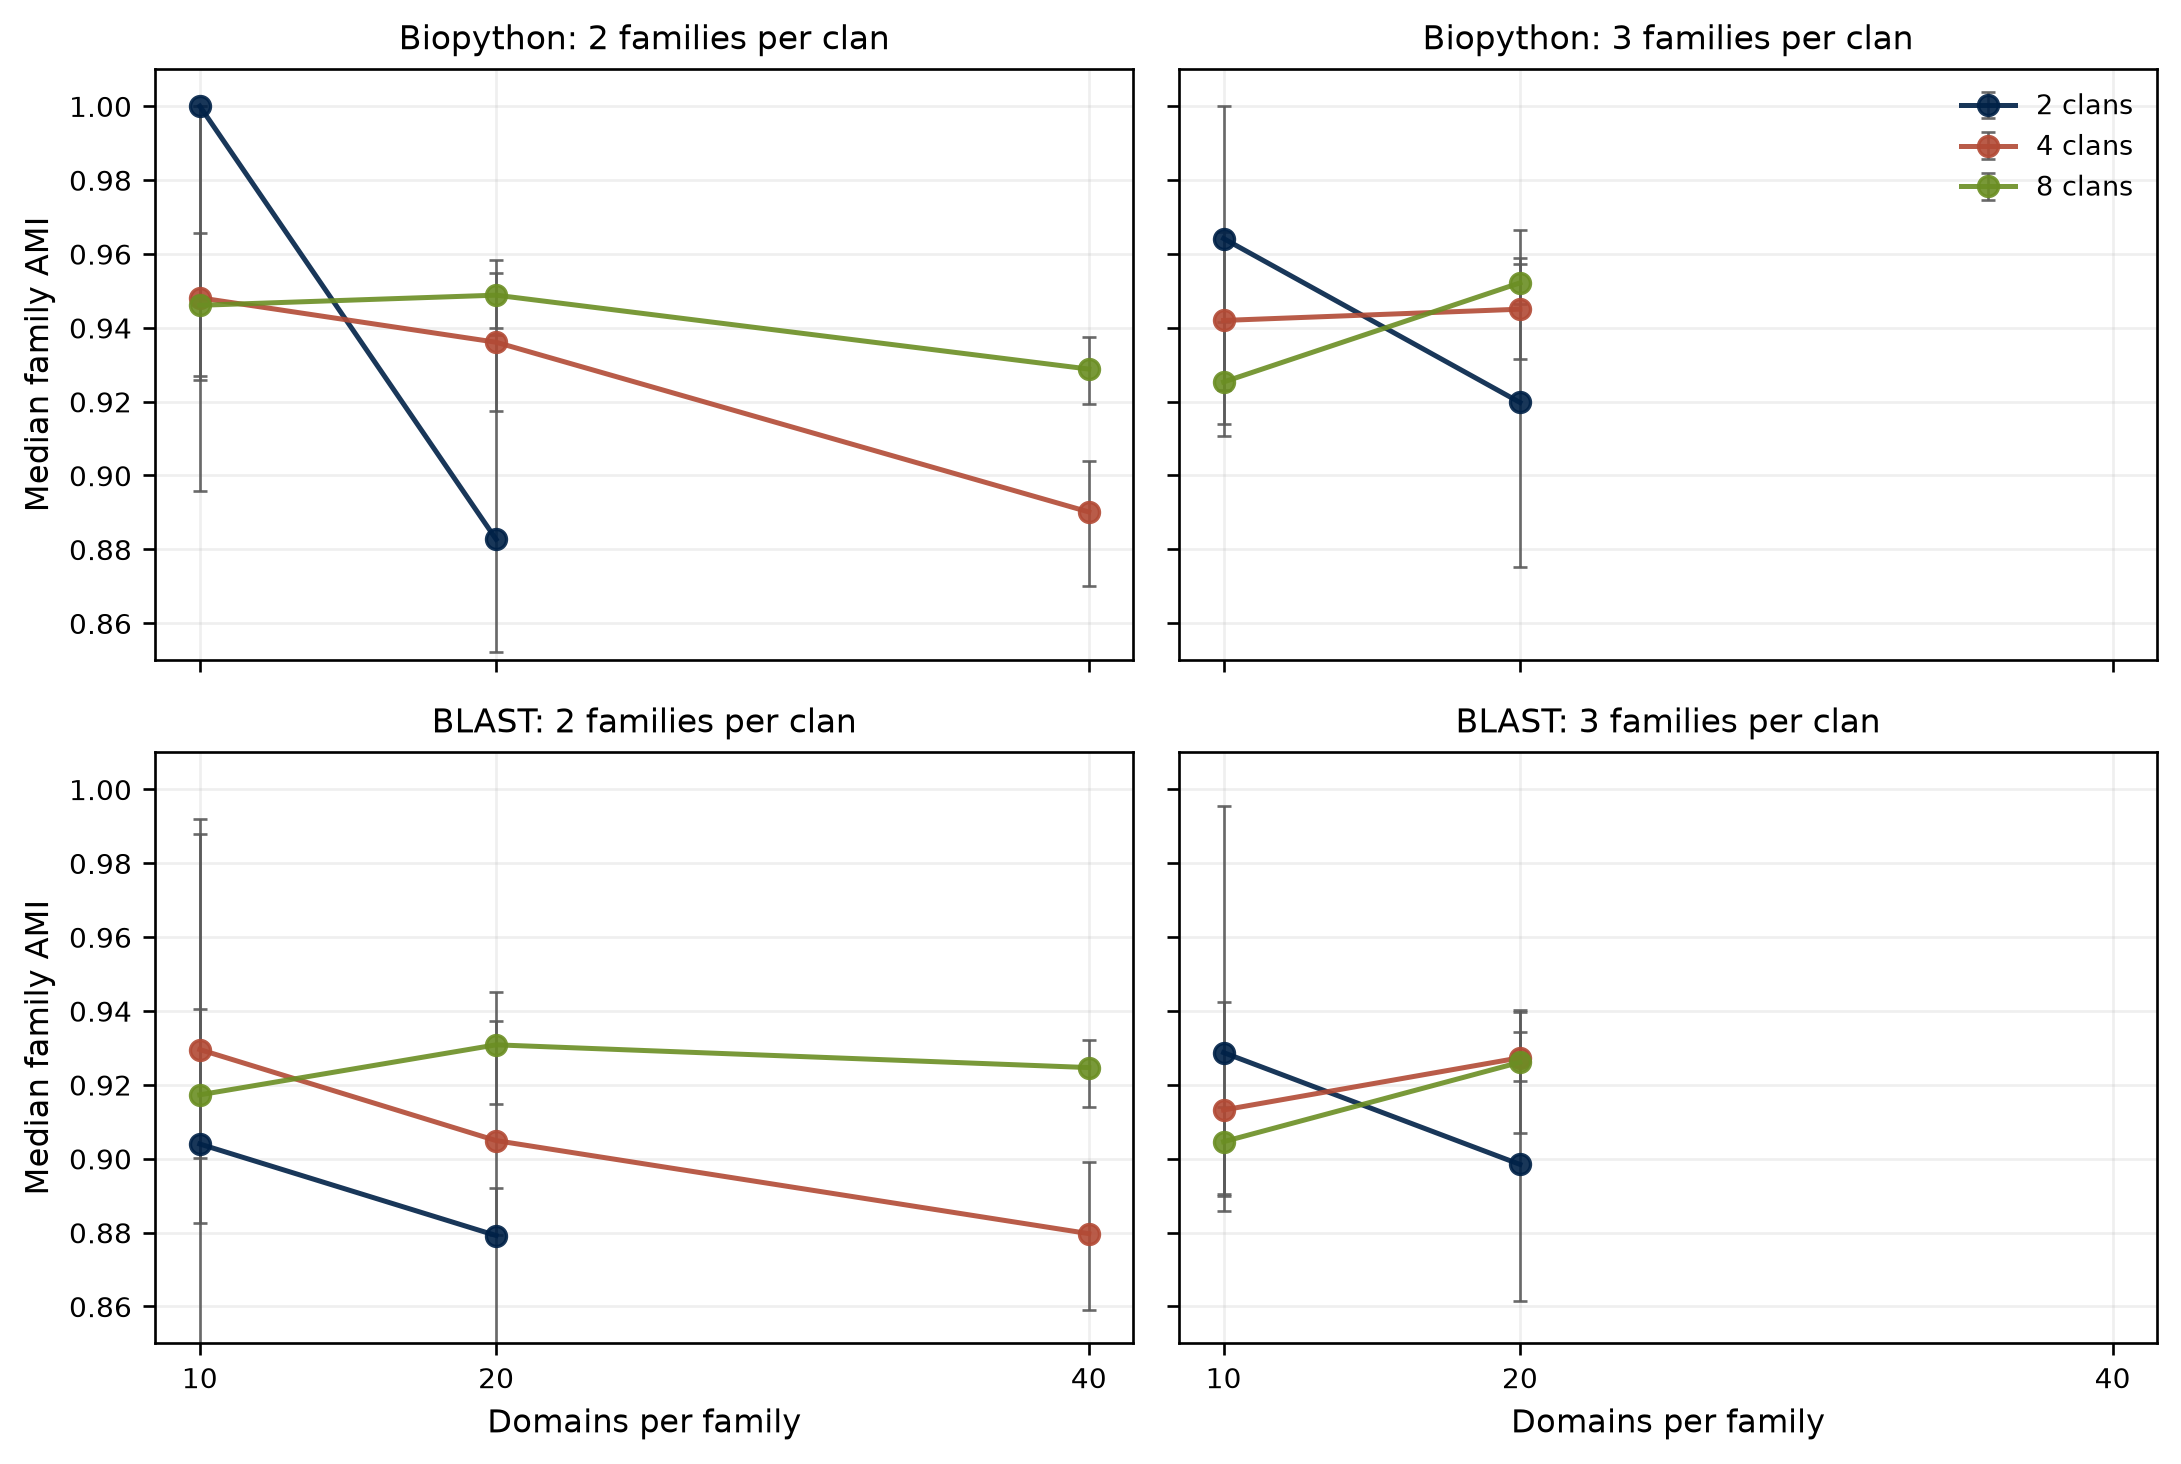
\includegraphics[width=\textwidth]{composition_recovery.png}
  \caption{Median family AMI across \PrimaryConditions\ primary composition
  conditions under top-5 construction, with interquartile ranges across
  collections as error bars. Colour gives clan count; panels separate
  score method and families per clan. Lines connect domain counts.}
  \label{fig:composition}
\end{figure}

For fixed \(k\), retained edge count grows at most linearly with vertex count
\(n\), while possible pair count grows as \(\binom n2\). Realised density
therefore decreased with collection size (Fig.~\ref{fig:composition-topology},
left). Median component count also varied with clan and family counts
(Fig.~\ref{fig:composition-topology}, right).

\begin{figure}[htbp]
  \centering
  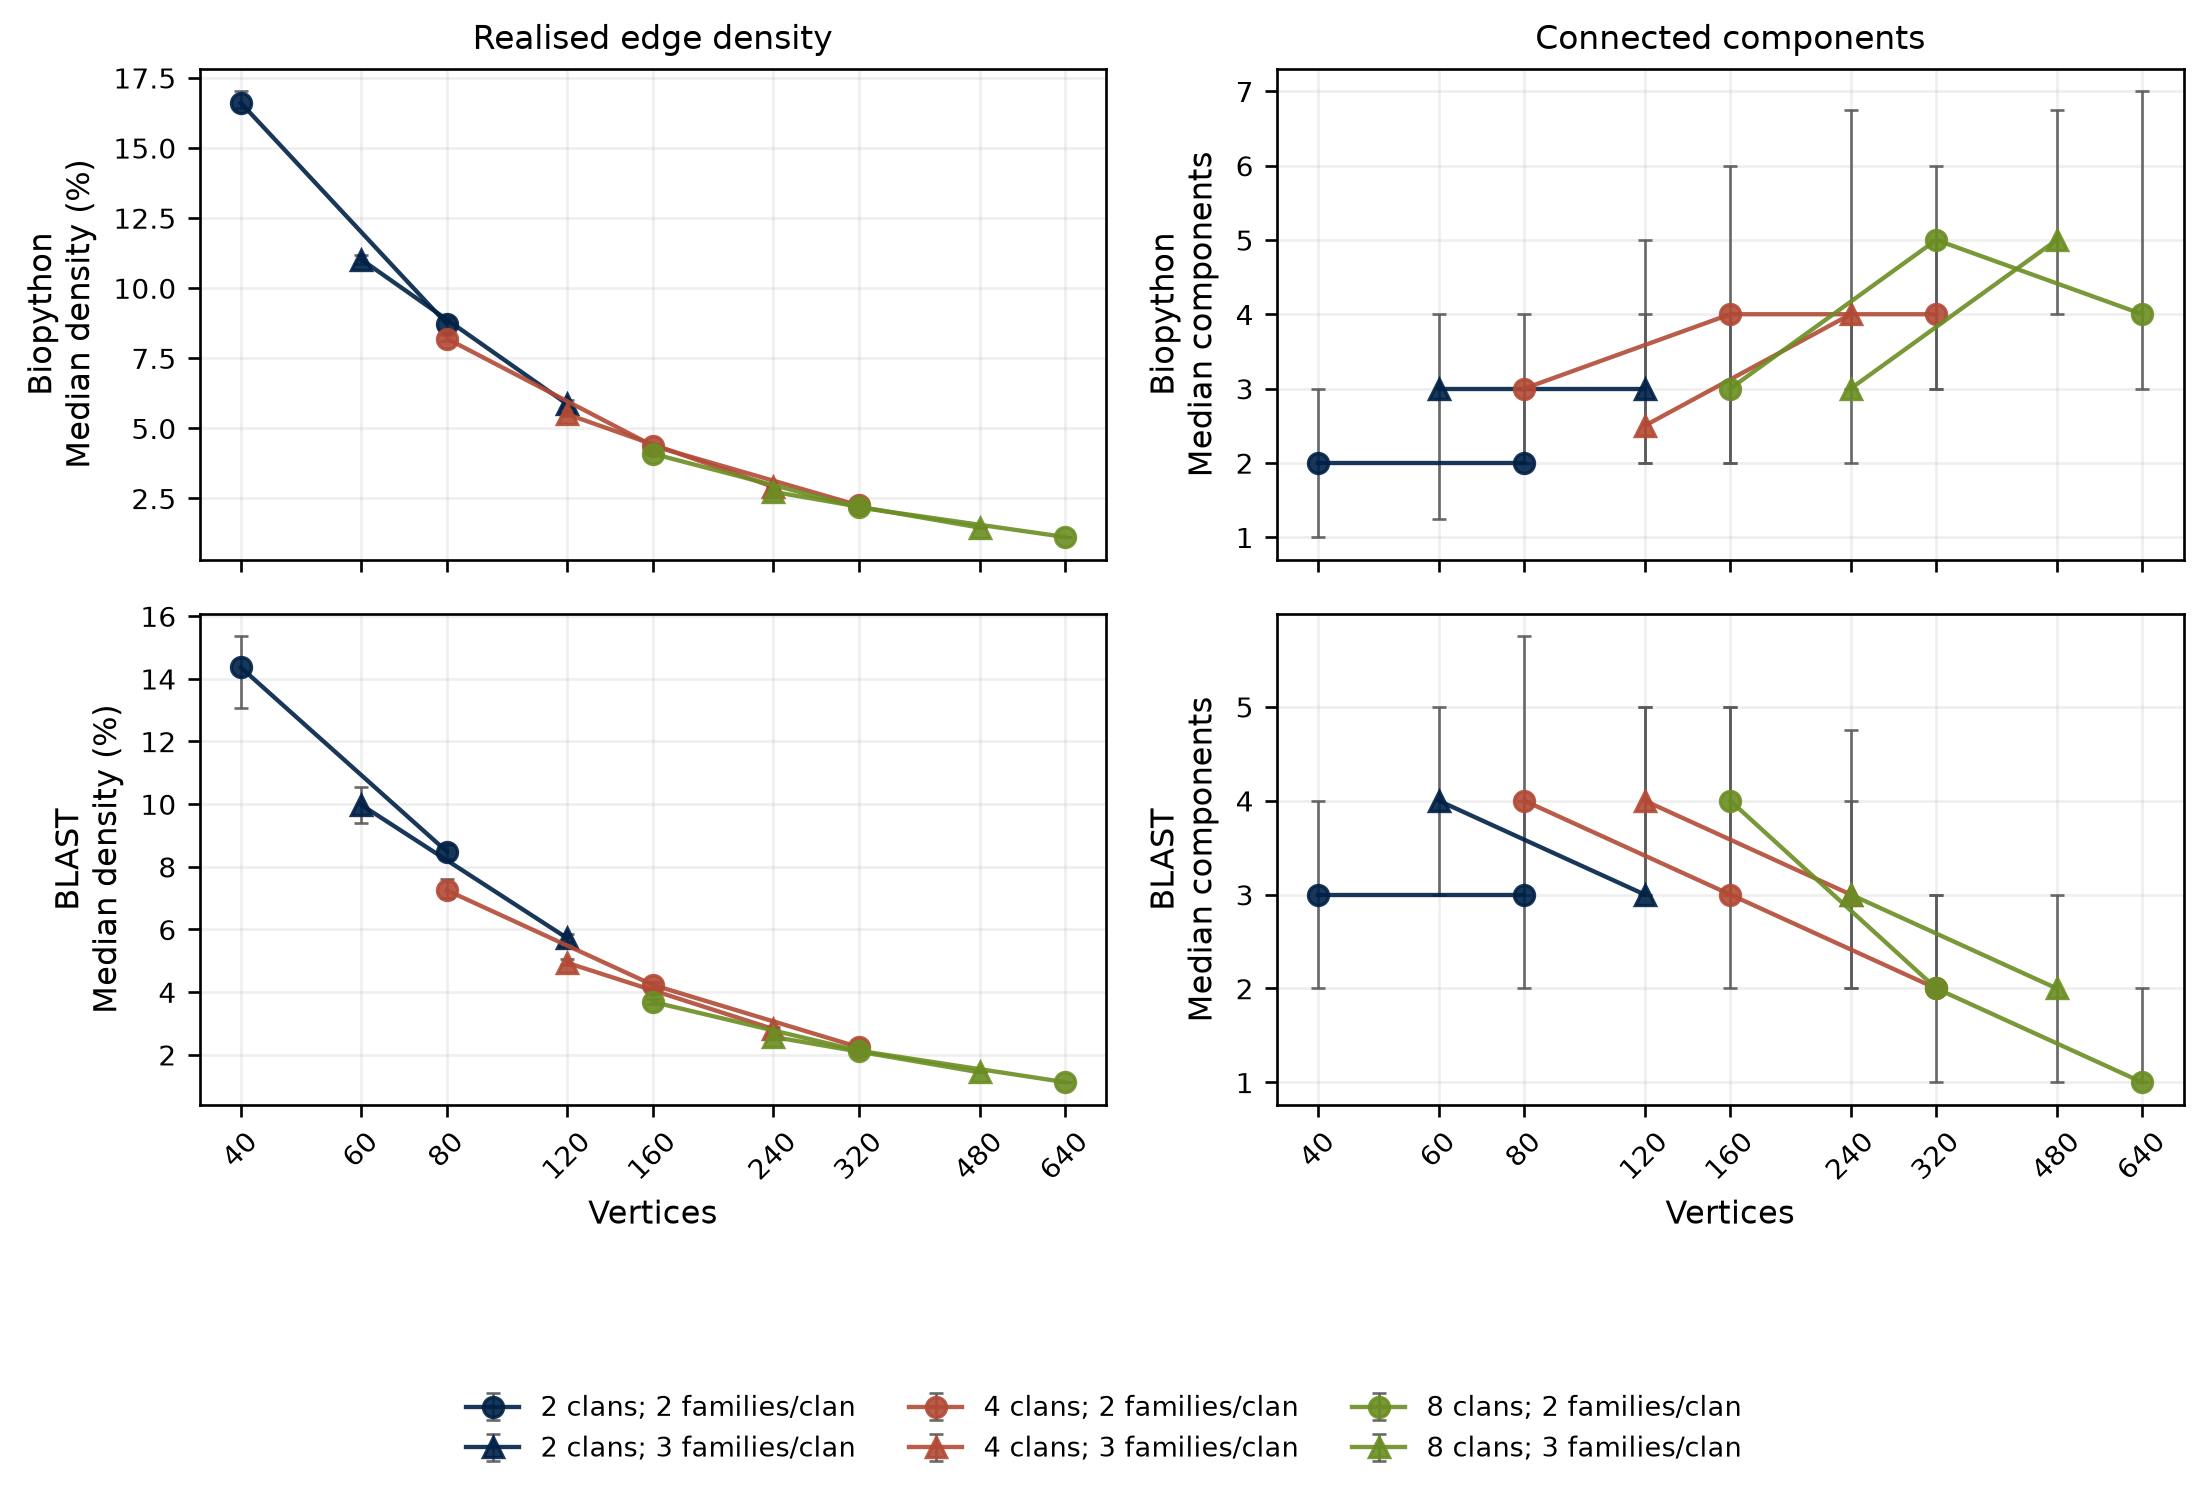
\includegraphics[width=\textwidth]{composition_topology.png}
  \caption{Top-5 graph structure across \PrimaryConditions\ primary
  composition conditions, with interquartile ranges across collections as error
  bars. Rows separate score methods. Colour gives clan
  count; marker gives families per clan, circle for two and triangle for three.
  Lines connect domain counts.}
  \label{fig:composition-topology}
\end{figure}

\subsection{Sensitivity analyses}

We permuted scores within each collection, which preserves the score
distribution and rule parameters while randomising pair identities. In reference condition,
Biopython top-5 median family AMI changed from \ObservedTopFiveAMI\ to
\NullTopFiveAMI\ (Fig.~\ref{fig:sensitivity}, left). Positive null NMI
confirmed chance bias in finite partitions addressed by AMI.

For unweighted Louvain, we replaced every retained edge weight by one. Reference
Biopython top-5 median family AMI was \UnweightedTopFiveAMI, compared with
\ObservedTopFiveAMI\ under native weights (Fig.~\ref{fig:sensitivity}, right).
Selected adjacency therefore retained family agreement after removal of edge
weight variation for this setting.

\begin{figure}[htbp]
  \centering
  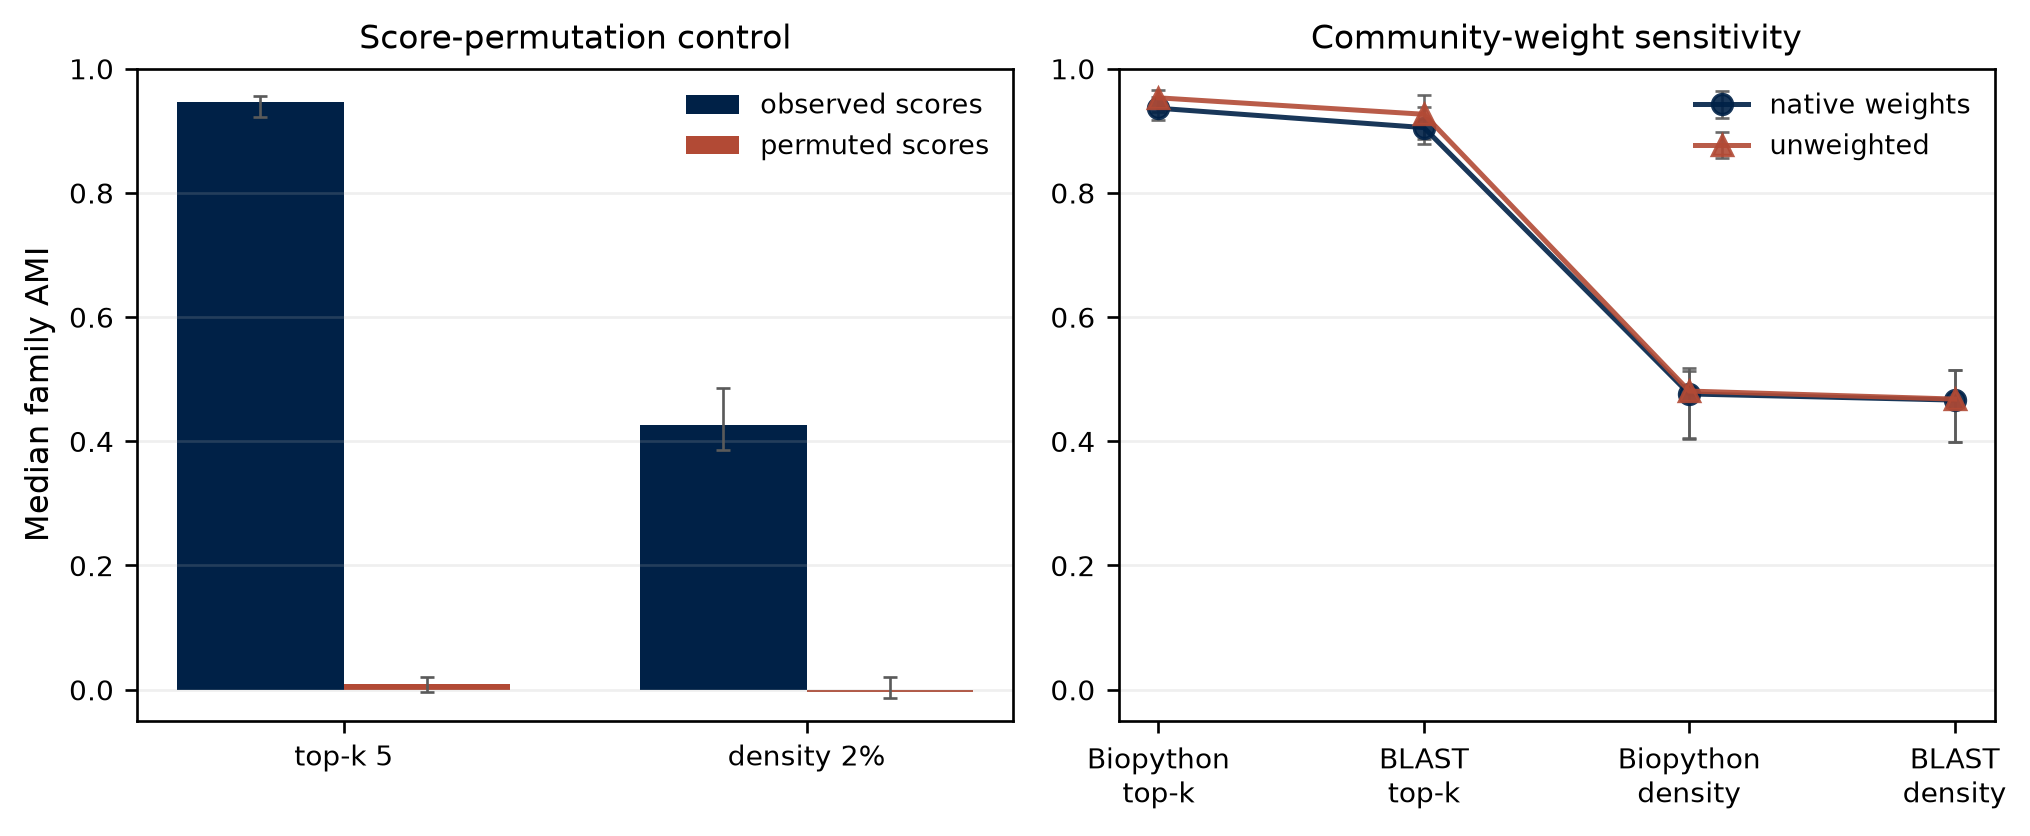
\includegraphics[width=\textwidth]{sensitivity_checks.png}
  \caption{Sensitivity to score permutation and community weight. Bars and
  markers give medians; error bars give interquartile ranges across
  collections.}
  \label{fig:sensitivity}
\end{figure}
\FloatBarrier

\section{Discussion}

\paragraph{Main finding.}
We found that top-\(k\) rules, which build a graph by connecting each protein
domain to the \(k\) domains with which it has the highest alignment scores,
recovered withheld Pfam labels most consistently across tested score methods
and label levels. Top-10 maximised median family AMI for both methods and was
within \TopTenClanAMIGap\ of the highest clan AMI. Top-5 retained fewer edges, with median
family AMI \BioTopFiveAMI\ for Biopython and \BlastTopFiveAMI\ for BLAST. We
found that both perform well, so the choice between them depends on the desired
graph sparsity.

\paragraph{Edge allocation.}
From our follow-up experiments on graph topology (Section~\ref{sec:sparsity}),
we believe that edge allocation explains much of this result. Sparse global
rules produced many components, whereas top-\(k\) produced fewer components at
similar density because each vertex selects local neighbours. Global density
alone therefore did not determine graph structure.

\paragraph{Agreement measure.}
We found that NMI exceeded AMI under sparse, fragmented settings
(Figs.~\ref{fig:nmi-frequency} and~\ref{fig:ami-frequency}). Because AMI
subtracts expected mutual information conditional on observed group sizes, we
used AMI for comparisons across rules and compositions, with NMI as an
unadjusted bounded descriptor.

\paragraph{Score method.}
Biopython and BLAST ranks agreed closely among pairs reported by BLAST, while
BLAST covered only \BlastCoveragePct\% of master pairs. Despite this low
coverage, BLAST top-\(k\) graphs recovered family labels nearly as well as
exact alignment, since BLAST reports concentrated among the highest-scoring
pairs (Fig.~\ref{fig:score-coverage}), which are the pairs top-\(k\) rules
select. Equal percentiles combined
score method, coverage, and edge-budget effects. Target density removed the
edge-budget difference; at 2\% density, median absolute family differences were
\MatchedTwoAbsDeltaNMI\ for NMI and \MatchedTwoAbsDeltaAMI\ for AMI. Agreement
between methods after density matching supports graph-rule conclusions shared
by both score systems.

\paragraph{Collection composition.}
Collection composition changed density, component count, and recovery under a
fixed top-5 rule. Balanced sampling estimates behaviour across controlled
mixtures rather than natural Pfam abundance. Replicate variation within each
condition captures domain and family selection effects for this master panel.

\paragraph{Controls.}
Our permutation control shows that pair identity carries family information
beyond the score distribution: permuting scores reduced reference family AMI
from \ObservedTopFiveAMI\ to \NullTopFiveAMI. With unit weights, family AMI at
the reference setting was \UnweightedTopFiveAMI, compared with
\ObservedTopFiveAMI\ under native weights. These controls locate the observed
signal primarily in edge placement rather than edge weights for this setting.

\paragraph{Limitations and future work.}
Inference scope remains balanced mixtures from \MasterFamilies\ selected Pfam
families. Full-length proteins, alternative databases, synthetic evolutionary
data, and structural labels require separate evaluation. \ExcludedCells\
saturated design conditions reduced primary factorial design to
\PrimaryConditions\ conditions. Louvain resolution and stochasticity received
limited study. DEDAL lacks scaled evidence here.
Future work should repeat sampling across broader Pfam panels, model composition
effects with hierarchical uncertainty, test graph filtrations across continuous
edge budgets, and compare community algorithms. These experiments estimate
stability across panels and graph construction choices.

\section{Conclusion}

In this project, we studied sequence-similarity networks, graphs built from
protein sequences using pairwise alignment scores. Our goal was to develop and
test a framework that evaluates how methodological choices in building SSNs
affect the biological relevance of the resulting networks. We built a pipeline
that maps recorded domain collections to pair scores, weighted graphs,
communities, and auditable agreement measures. Among tested settings, we found
that top-\(k\) rules recovered withheld Pfam structure most consistently; top-10 maximised
family AMI and top-5 supplied a sparser alternative with median family AMI of
at least \TopFiveMinFamilyAMI\ under both score methods. AMI corrected
chance agreement caused by variable community counts. Biopython and BLAST
produced similar recovery after edge budgets were matched, while equal
percentiles produced different graph densities. Sampling frame, score coverage,
edge rule, and realised density should accompany each reported SSN result.

\clearpage
\appendix

\section{Panel selection algorithm}
\label{app:panel}

Parameters used were \(c^\ast=\MasterClans\), \(f^\ast=3\),
\(r^\ast=\TargetPerFamily\), and \(\sigma=\SamplingSeed\).

\begin{algorithm}[htbp]
\setstretch{1}
\caption{Seeded selection of clan and family panel}
\label{alg:panel}
\begin{algorithmic}[1]
  \Require catalogue of Pfam families with clan assignment; targets \(c^\ast\) clans and \(f^\ast\) families per clan; minimum reported seed count \(r^\ast\); seed \(\sigma\)
  \Ensure panel of \(c^\ast f^\ast\) families, and trace of every family inspected
  \State \(\mathcal C\gets\) clans holding at least \(f^\ast\) catalogue families, excluding unassigned
  \State sort \(\mathcal C\), then shuffle under \(\sigma\)
  \State \(P\gets\emptyset\)
  \ForAll{\(C\in\mathcal C\) in shuffled order}
    \State sort families of \(C\), then shuffle under same stream
    \State \(A\gets\emptyset\)
    \ForAll{\(F\) in shuffled families of \(C\)}
      \State query InterPro for entry type and reported seed count of \(F\)
      \State append \(F\) to trace
      \If{type of \(F\) is \emph{domain} or \emph{family}, and seed count \(\geq r^\ast\)}
        \State \(A\gets A\cup\{F\}\)
      \EndIf
      \If{\(\lvert A\rvert=f^\ast\)} \State \textbf{break} \EndIf
    \EndFor
    \If{\(\lvert A\rvert=f^\ast\)}
      \State \(P\gets P\cup A\) \Comment{otherwise clan \(C\) is skipped}
      \If{\(P\) spans \(c^\ast\) clans} \State \textbf{break} \EndIf
    \EndIf
  \EndFor
  \State \Return \(P\) and trace
\end{algorithmic}
\end{algorithm}

\footnotesize
\setlength{\bibsep}{1pt}
\bibliographystyle{abbrvnat}
\bibliography{references}

\end{document}
